\documentclass[a4paper,ngerman,oneside,titlepage,bibliography=totoc,11pt]{scrreprt}


\pagestyle{headings}

\usepackage{geometry}
\geometry{left=31mm, top=34mm, right=31mm, bottom=34mm}

\renewcommand{\ttdefault}{lmtt}
\linespread{1.06} %font

\usepackage[font=small,labelfont=bf]{caption} %caption, caption-font
\usepackage{subcaption}
\usepackage{amsmath, amsthm, amssymb, amsbsy}
\usepackage{mathtools}
\usepackage{color}
\usepackage{booktabs}
\usepackage{microtype}
\usepackage{natbib}
\usepackage[ngerman]{babel}
\usepackage[utf8]{inputenc} % für Umlaute (ansinew Editor, utf8 bei Texniccenter/Texmaker)
\usepackage[T1]{fontenc} % korrekte Trennung von Umlauten

\usepackage{lmodern}
\usepackage[hyphens]{url}
\usepackage{hyperref}
\usepackage{animate}
\usepackage{rotating}
\usepackage{longtable}
\usepackage{setspace}
\onehalfspacing



\begin{document}



\begin{titlepage}

\newcommand{\HRule}{\rule{\linewidth}{0.5mm}} % Defines a new command for the horizontal lines, change thickness here

\center % Center everything on the page
 
%----------------------------------------------------------------------------------------
%	HEADING SECTIONS
%----------------------------------------------------------------------------------------

\LARGE Ludwig-Maximilians-Universität München\\[0.2cm] % Name of your university/college
\LARGE Institut für Statistik\\[5mm]% Major heading such as course name
\large Projekt im Rahmen des statistischen Consultings\\[6mm]
% Minor heading such as course title

%----------------------------------------------------------------------------------------
%	TITLE SECTION
%----------------------------------------------------------------------------------------

\HRule \\[0.4cm]
{ \huge \bfseries Internationaler Waffenhandel:\vspace{-1.5mm} Die Anwendung neuer Verfahren der\\[1mm] statistischen Netzwerkanalyse}\\[5mm]
{ Eine Netzwerkanalyse des internationalen Kleinwaffenhandels 1992 - 2011}\\
{ Kooperation mit dem Lehrstuhl für empirische Politikforschung}\\[0.4cm] % Title of your document
\HRule \\[1.5cm]
 
%----------------------------------------------------------------------------------------
%	AUTHOR SECTION
%----------------------------------------------------------------------------------------

\begin{minipage}[t]{0.4\textwidth}
\begin{flushleft} \large
\emph{Autor:}\\[2mm]
Felix Loewe\\
loewe.felix@gmail.com\\[5mm]


\end{flushleft}
\end{minipage}
~
\begin{minipage}[t]{0.4\textwidth}
\begin{flushright} \large
\emph{Projektpartner:}\\[2mm]
Prof. Dr. Paul W. Thurner\\[6mm]

\emph{Betreuer:}\\[2mm]
Prof. Dr. Göran Kauermann\\[6mm]
\end{flushright}
\end{minipage}\\[4.5cm]

\end{titlepage}




\begin{abstract}


\begin{center}
{\it \bf Abstract} 
\end{center}

\noindent
Die \emph{NISAT Database} des \emph{Peace Research Institute Oslo (PRIO)} enthält Daten über den internationalen Handel mit Kleinwaffen und Leichtwaffen von insgesamt 239 verschiedenen Ländern im Zeitraum von 1992 bis 2011. Diese wurden mit neuen Methoden der statistischen Netzwerkanalyse untersucht.\\

\noindent
Im Rahmen des Projekts wurde zunächst eine deskriptive Analyse durchgeführt, die unter anderem zentrale Akteure des Netzwerkes identifizieren konnte. Ein besonderes Augenmerk galt hier der Veränderung der Netzwerkstrukturen über die Zeit. Anschließend wurde mit Hilfe zusätzlicher Kovariablen versucht, ein \emph{Exponential Random Graph Model (ERGM)} auf die Netzwerkdaten der einzelnen Jahre anzupassen. Die Ergebnisse der Modellierung wurden abschließend mit denen eines vorhergehenden Projekts über den Handel mit Großwaffen verglichen.
 


\end{abstract}




\tableofcontents




\chapter{Einleitung}
Die statistischen Methoden der Netzwerkanalyse finden ein breites Anwendungsfeld. Neben klassischen Anwendungen wie in den Sozialwissenschaften (z.B. Freundesnetzwerk, Kollegenkreis)  und Politikwissenschaften (z.B. internationale Beziehungen) ist sie auch in modernen Bereichen der Informatik (Computernetzwerk, soziale Netzwerke im Internet) und der Biologie (Proteinverbindungen der menschlichen DNA) von großem Nutzen.

Was ist jedoch das Besondere an der statistischen Analyse von Netzwerken? Durch ihre Abhängigkeitsstruktur stellen sie relationale Daten dar. Gewöhnliche Datensätze werden in der Statistik zumeist mit der Annahme analysiert, dass die Beobachtungen als unabhängig voneinander betrachtet werden können. Bei Netzwerkdaten ist das nicht der Fall. Hier stehen die Beobachtungen, oft genannt \emph{Akteure} des Netzwerkes, in einer Beziehung zueinander, die bei der Analyse der Daten  selbst von zentralem Interesse ist. Besteht jedoch eine Beziehung zwischen den Beobachtungen, können diese nicht mehr als unabhängig angesehen werden, was alternative Methoden der statistischen Modellierung erfordert. 

Das Bestehen oder Nicht-Bestehen einer Beziehung bezeichnet man als die Netzwerkstruktur (Abhängigkeitsstruktur), die zusätzlich zu den Daten eines gewöhnlichen Datensatzes besteht. Die Abhängigkeitsstruktur wird durch die \emph{Adjazenzmatrix} $A_{ij} \in N \times N$ ausgedrückt.

Gegenstand der Analyse in dieser Arbeit ist ein Datensatz zum internationalen Handel mit kleinen und leichten Waffen. 
Bei der Analyse des Waffenhandels wird aus den Akteuren die exportierenden oder importierenden Länder und aus deren Abhängigkeit ein Handel.

Die Arbeit ist wie folgt aufgebaut: Im ersten Kapitel erfolgt eine kurze Einführung in die Grundlagen der Graphentheorie. Netzwerkspezifische Begriffe sowie deskriptive Maßzahlen werden definiert. Darauf folgt eine Erläuterung der Datengrundlage der NISAT Datenbank mit den daraus resultierenden Möglichkeiten und Einschränkungen. Im dritten Abschnitt wird der Datensatz deskriptiv analysiert. Darauf aufbauend folgt im vierten Abschnitt die Modellierung per ERGM. Im Anschluss werden die Ergebnisse der vorhergehenden Analyse mit denen einer ähnlichen Arbeit über den Handel mit Großwaffen verglichen. Im letzten Abschnitt werden die erarbeiteten Ergebnisse zusammengefasst und diskutiert.





\chapter{Zusammenfassung der Graphentheorie}

Um Netzwerkdaten statistisch analysieren zu können, muss die Abhängigkeitsstruktur der Daten adäquat modelliert werden. Eine grundlegende mathematische Theorie, die verwendet wird, um \emph{relationale Daten} zu beschreiben, ist die Graphentheorie. Im Rahmen dieses Kapitels wird nur auf die wichtigsten Aspekte der Graphentheorie eingegangen. Es handelt sich im Wesentlichen um eine Zusammenfassung der Kapitels 2.1 und 4.2 aus \citet{kol09}.

\section{Graph - Grundlegende Begriffe}

Ein \emph{Graph} $G = (V,E)$ ist die mathematische Beschreibung eines Netzwerkes. Er besteht aus einer Knotenmenge $V$ und einer Kantenmenge $E$. Ein \emph{Knoten} repräsentiert einen Akteur des Netzwerkes. Eine \emph{Kante} verbindet zwei Akteure und kennzeichnet eine Beziehung zwischen ihnen.

Die Anzahl der Knoten $N_V = |V|$ wird üblicherweise als kleiner unendlich vorausgesetzt. Häufig benennt man die Knoten eines Netzwerkes einfach nach ihren Index $i = 1, ..., N_V$.

Eine Kante $\{i,j\}$ ist ein Element der Menge $E$ und  beschreibt die Verbindung zwischen Knoten $i$ und $j$.

Man unterscheidet zwischen \emph{gerichteten} und \emph{ungerichteten} Graphen. Ein ungerichteter Graph setzt eine symmetrische Beziehung zwischen den Akteuren voraus. Akteur $i$ steht also zu Akteur $j$ in der gleichen Beziehung wie $j$ zu $i$ (z.B. Facebook Freundschaft). Bei einem gerichteten Graphen hingegen ist die Richtung der Beziehung entscheidend. Dies ist im hier betrachteten Datensatz der Fall. Man unterscheidet zwischen Exporteur und Importeur eines Handels. Die Kante $\{i,j\}$ ist hier also von der Kante $\{j,i\}$ zu unterscheiden. Einen gerichteten Graphen nennt man auch \emph{Digraph}.

Per Definition enthält ein Graph weder Schleifen noch multiple Kanten. Von einer \emph{Schleife} spricht man, wenn eine Kante $\{i,j\}$ den gleichen Anfangs- und Endpunkt besitzt ($i = j$). Von einer \emph{multiplen Kante} spricht man, falls zwischen zwei Knoten mehrere Verbindungen bestehen. Enthält ein Netzwerk solche Eigenschaften, spricht man von einem \emph{Multigraphen} ansonsten von einem \emph{einfachen Graphen}.

Betrachtet man die Anzahl der möglichen Kanten eines Graphen, die später als Benchmark dafür auftaucht, wie dicht ein Graph sein kann, so wird ersichtlich, dass diese Anzahl für einen einfachen ungerichteten Graphen kleiner ist als die Anzahl der möglichen Kanten eines gerichteten Graphen. Für einen einfachen ungerichteten Graphen ist sie gegeben durch $V_H(V_H-1)/2$. Ein gerichteter Graph kann logischerweise maximal die doppelte Anzahl an Kanten enthalten.

Notwendigerweise gibt es einige Begriffe, um über die Konnektivität von Graphen zu reden. Am gebräuchlichsten ist das Prinzip der \emph{Nachbarschaft}. Zwei Knoten $ i,j \in V$ gelten als benachbart, wenn sie von einer Kante $\{i,j\} \in E$ verbunden werden. Zwei Kanten wiederum gelten als benachbart, wenn beide einen gemeinsamen Knoten aus $V$ enthalten.

Ein sogenannter \emph{Weg} auf einem Graphen von $v_0$ nach $v_l$ bezeichnet die alternierende Sequenz $\{v_0, e_1, v_1, e_2, ..., v_{l-1}, e_l, v_l\}$. $l$ bezeichnet hierbei die Länge des Weges. Weiter beschreibt ein \emph{Pfad} einen Weg ohne wiederholte Knoten oder Kanten. Als \emph{Distanz} zwischen zwei Knoten eines Graphen definiert man die Länge des kürzesten Pfades, der sie verbindet. Die Länge der längsten Distanz innerhalb eines Graphen nennt man den \emph{Durchmesser} oder \emph{Diameter} eines Graphen.

Soviel zu den grundlegenden Begrifflichkeiten der Graphentheorie. Mit ihrer Hilfe werden nun in den folgenden Unterpunkten einige für die folgenden Analysen besonders wichtige Definitionen erläutert.

\section{Degree-Verteilung}
Ein weiterer Begriff ist der des \emph{Degree} eines Knotens $d_v$, definiert als die Anzahl der Kanten, die den Knoten $v$ enthalten. Die \emph{Degree-Sequenz} eines Graphen ist die Sequenz, die entsteht, wenn man alle Knoten-Degrees in aufsteigender Reihenfolge sortiert. Nun definiert man $f_d$ als den Anteil der Knoten $v \in V$ mit Degree $d_v = d$. Die Reihe $\{f_d\}_{d \geq 0}$ heißt \emph{Degree-Verteilung} von $G$. 

Bei einem gerichteten Graphen unterscheidet man zwischen \emph{In-Degree} ($d_v^{in}$) und \emph{Out-Degree} ($d_v^{out}$) und zählt nur die Kanten, die zu einem Knoten hin beziehungsweise von ihm weg laufen. Die eben genannten Begriffe lassen sich hierfür trivial erweitern.

\section{Nachbarschaftsmatrix}

Die Struktur eines Graphen ist vollständig bestimmt durch seine binäre und symmetrische\emph{ Nachbarschaftsmatrix} (auch \emph{Adjazenzmatrix}) $A \in |N_V| \times |N_V|$, wobei $a_{ij} = 1$, falls zwischen Knoten $i$ und Knoten $j$ eine Kante besteht und $a_{ij} = 0$ sonst. Diese Matrix hat einige nützliche Eigenschaften. Zum Beispiel ergibt die Zeilensumme $A_{i,} = \sum_j{A_{ij}}$ den Degree $d_i$ von Knoten $i$.  
Bei gerichteten Graphen besteht ein Unterschied zwischen der Kante $(i,j)$ und der Kante $(j,i)$. Die Adjazenzmatrix ist hier also nicht symmetrisch. Allerdings enthält sie immer noch ähnliche Informationen wie zum Beispiel $A_{i,} = d_i^{out}$ und $A_{,j} = d_j^{in}$.

\section{Zentralität}
Viele Fragestellungen der Netzwerkanalyse drehen sich darum, welche Akteure auf eine bestimmte Weise besonders wichtig für ihr Netzwerk sind. Maßzahlen der Zentralität sind dafür gedacht, die Wichtigkeit der Knoten zu quantifizieren und dadurch die Beantwortungen solcher Fragestellungen zu vereinfachen. Das wichtigste Konzept in diesem Zusammenhang, den Degree, haben wir bereits kennen gelernt. Zusätzlich werden nun kurz die Begriffe Closeness- und Betweeness Zentralität eingeführt.

Bei der \emph{Closeness} Zentralität wird ein Knoten als zentral angesehen, falls er vielen anderen Knoten "`nahe"' ist.
Man verwendet für dieses Maß die Inverse der Summe der Distanzen eines Knotens zu allen anderen,
$$ c_{Cl}(v)=\frac{1}{\sum_{u \in V}{dist(v,u)}}, $$
wobei $dist(v,u)$ die Distanz zwischen den Knoten $v$ und $u$ bezeichnet. Um eine Vergleichbarkeit mit anderen Graphen und Zentralitätsmaßen herzustellen, normalisiert man die Maßzahl in das Intervall $[0,1]$, indem man mit dem Faktor $N_v - 1$ multipliziert.

Ein anderes Konzept basiert auf dem Gedanken, dass die Wichtigkeit eines Knotens darauf beruht, wie oft sich ein Knoten auf der Verbindung zwischen anderen Paaren von Knoten befindet. Knoten, die auf vielen Pfaden eines Netzwerkes sitzen, werden als wichtig für die Kommunikation innerhalb des Netzwerkes angesehen. 
Die \emph{Betweeness} Zentralität wird deswegen üblicherweise definiert als
$$ c_{B}(v)= \sum_{s \neq t \neq v \in V} {\frac{\sigma(s,t|v)}{\sigma(s,t)}}, $$
wobei $\sigma(s,t|v)$ die Anzahl der kürzesten Pfade zwischen $s$ und $t$ ist, die durch $v$ verlaufen und $\sigma(s,t) = \sum_v{\sigma(s,t|v)}$.

\section{Dichte}
Die \emph{Dichte} eines Netzwerkes ist die Anzahl der Kanten des Netzwerkes, geteilt durch die mögliche Anzahl an Kanten des Netzwerkes. Es ergibt sich der Term $$den(G) = \frac{|E_G|}{|V_G|(|V_G|-1)/2}$$ für die Dichte eines ungerichteten Netzwerkes und $$den(G) = \frac{|E_G|}{|V_G|(|V_G|-1)}$$ für ein gerichtetes Netzwerk. Die Dichte liegt zwischen null und eins. Es sei angemerkt, dass die Dichte auch als Skalierung des durchschnittlichen Degrees $\bar{d}(G)$ angesehen werden kann, denn $den(G) = (|V_G| - 1) \bar{d}(G)$.

\chapter{Datengrundlage}
Die Datengrundlage für das Kleinwaffenhandelsnetzwerk ist die \emph{NISAT} (Norwegian Initiative on Small Arms Transfers) Datenbank. Das Peace Research Institute Oslo (PRIO) ist der Auftraggeber dieser Datenbank. Das Institut hat es sich zur Aufgabe gemacht, "`[...] die Bedingungen, die ein friedliches Zusammenleben zwischen Staaten, Gruppen und Menschen [..]"' \footnote{\URL{https://www.prio.org/}} ermöglichen, zu erforschen. Die Datenbank enthält Daten über den Handel von kleinen und leichten Waffen. Der abgedeckte Zeitraum beträgt die Jahre 1992 bis 2011. Berichtet wird hierin von insgesamt 239 Ländern und 109522 Waffentransaktionen.

Die Daten liegen in der Form einer gerichteten Kantenliste vor. Das bedeutet, jede Zeile im Datensatz entspricht einem Handel zwischen einem exportierenden und einem importierenden Land. Zusätzliche Attribute sind der Correlates of War Code des jeweiligen Landes, der monetäre Wert des Handels in US Dollar, der gehandelte Waffentyp , die berichtende Datenquelle sowie das Jahr, in dem der Handel stattgefunden hat.

Bei der Betrachtung dieser Daten fallen folgende Probleme auf:
Da nach Waffentypen unterschieden wird, existieren in den einzelnen Jahren multiple Kanten. Das bedeutet, zwischen zwei Ländern werden im gleichen Jahr mehrere Transaktionen mit der gleichen Richtung aufgeführt. Diese wurden für die weitere Analyse zusammengefasst, indem der Wert der Lieferungen addiert wurde.

Der Datensatz enthält Schleifen. Das bedeutet, er enthält Zeilen, in denen der Exporteur und der Importeur eines Handels übereinstimmen. Da es hierfür keine sinnvolle inhaltliche Erklärung gibt, wurden die entsprechenden Beobachtungen gelöscht. Eine Liste der gelöschten Kanten befindet sich im elektronischen Anhang.

\chapter{Deskriptive Analyse}
Durch eine ausführliche deskriptive Analyse sollen Strukturen und Besonderheiten des vorliegenden Datensatzes herausgearbeitet werden. Von besonderem Interesse ist hierbei die zeitliche Komponente. Hierzu werden deskriptive Maßzahlen, Handelswerte und die Degree- Verteilungen für die 20 im Datensatz enthaltenen Jahre verglichen, um etwaige strukturelle Veränderungen des Netzwerkes zu erkennen.
Ein weiterer Teil befasst sich damit, die wichtigsten Akteure des Netzwerkes zu identifizieren. Zuletzt wird versucht, das Netzwerk zu visualisieren.

\section{Deskriptive Netzwerkmaßzahlen}
\begin{figure}[ht]
	\centering
		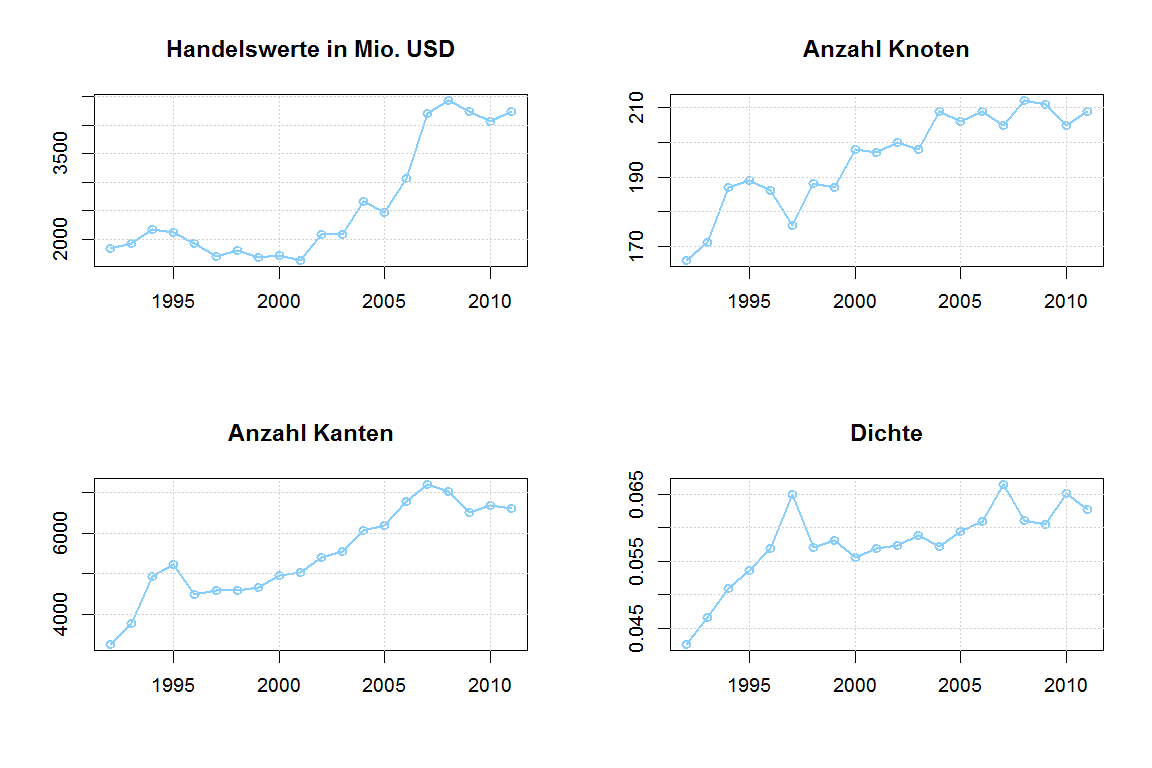
\includegraphics[width=0.9\textwidth]{Grafiken/ts_descriptives.png}
	\caption{Deskriptive Maßzahlen des Kleinwaffenhandelsnetzwerkes 1992 bis 2011}
	\label{fig:ts_descriptives}
\end{figure}
Zunächst erfolgt eine Darstellung grundlegender deskriptiver Netzwerkmaßzahlen, die das Kleinwaffenhandelsnetzwerk beschreiben. Die Maßzahlen werden für jedes Jahr berechnet und als Zeitreihe dargestellt, um die zeitliche Entwicklung des Netzwerkes zu visualisieren. Abbildung \ref{fig:ts_descriptives} zeigt die zeitliche Entwicklung von Handelswert, Knotenanzahl, Kantenanzahl und Dichte des Netzwerkes.

Betrachtet man zuerst die Zeitreihe der Handelswerte, so stellt man fest, dass diese in den Jahren 1992 bis 2001 relativ konstant zwischen 1.5 und 2.5 Milliarden US Dollar verweilt, nach 2001 jedoch bis auf circa 4.5 Milliarden im Jahr 2008 ansteigt und anschließend auf diesem Level konstant bleibt.

Die Zeitreihe der Anzahl der am Waffenhandel beteiligten Nationen steigt recht gleichmäßig zwischen den Jahren 1992 und 2011. Lediglich zwischen 1993 und 1994 ist ein außergewöhnlich starker Anstieg von 170 auf 187 zu beobachten. Im Jahr 1997 ist die Anzahl der am Waffenhandel beteiligten Nationen auffallend von 186 auf 176 gesunken. Allerdings stellt sich gleich im Folgejahr wieder die ursprüngliche Anzahl ein. Das Maximum der Zeitreihe liegt mit 212 Nationen im Jahr 2008.

Auch die Anzahl der Netzwerkkanten, also die Anzahl der vollzogenen Waffentransaktionen, zeigt einen regelmäßig steigenden Trend von circa 3000 im Jahr 1992 bis circa 7000 im Jahr 2011. Auch hier erkennen wir einen sprunghaften Anstieg zwischen 1993 und 1994 sowie ein Einknicken im Jahr 1996.
Die Dichte des Netzwerkes steigt in den Jahren 1992-1997 rasch von circa 0.04 auf 0.065 und schwankt  anschließend auf einem Level zwischen 0.055 und 0.065.

\section{Die Degree-Verteilung}

\label{sec:degree}
\begin{figure}[ht]
	\centering
		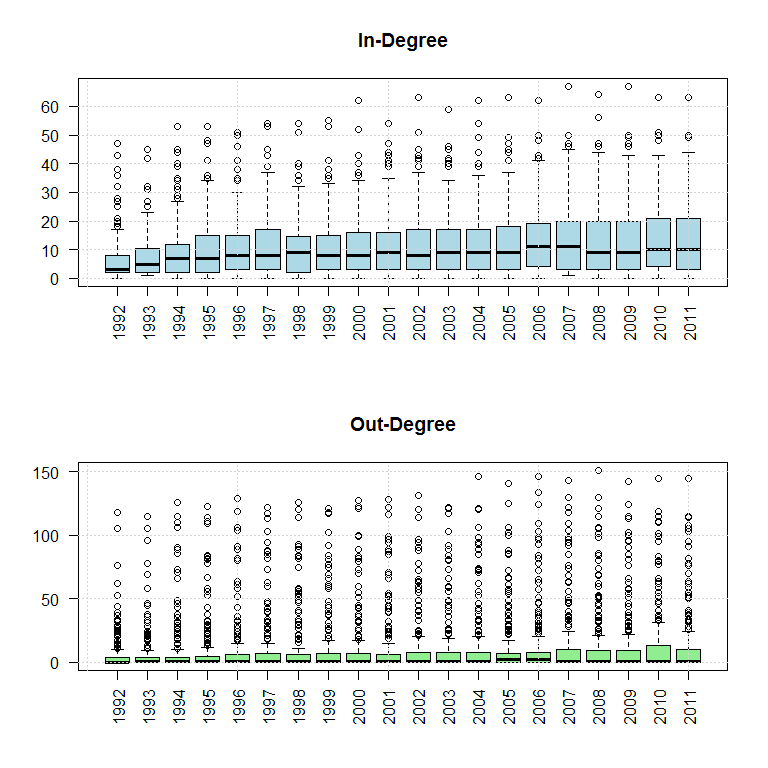
\includegraphics[width=1.00\textwidth]{Grafiken/ts_degree.png}
	\caption{Boxplot für In- und Out-Degree in den Jahren 1992 bis 2011}
	\label{fig:ts_degree}
\end{figure}

Eine erste nützliche Analyse, um die Struktur des Netzwerkes zu erfassen, ist die Betrachtung der Knoten-Degrees. Im Falle eines gerichteten Netzwerkes unterschiedet man zwischen In-Degree und Out-Degree. Inhaltlich interpretiert entspricht dies den Anzahlen der Importe und Exporte eines Landes. Hierzu betrachten wir die Abbildung \ref{fig:ts_degree}. Sie zeigt zu jedem im Datensatz enthaltenen Jahr je einen Boxplot der In-Degrees und Out-Degrees aller Länder. Innerhalb der farblich gekennzeichneten Box liegen jeweils die mittleren 50 Prozent der entsprechenden Daten. Der mittlere schwarze Strich in jeder Box kennzeichnet den Median und damit den Wert, unter dem genau die Hälfte aller Werte liegen.

Betrachtet man zuerst die Boxplots zum In-Degree, so stellt man fest, dass die Breite der Box über die Jahre zunimmt. Im Jahr 1992 reicht sie lediglich von zwei bis acht, während sie sich im Jahr 2011 von drei bis 21 erstreckt. Auch der Median steigt über diesen Zeitraum von drei auf zehn. Daraus lässt sich schließen, dass die mittlere Anzahl an Importpartnern eines einzelnen Landes über die Zeit größer geworden ist. Auffallend sind in allen Jahren einige mit Kreisen markierte Ausreißer, die aus bis zu 67 verschiedenen Ländern im gleichen Jahr Waffen beziehen.

Bei den Boxplots zum Out-Degree fallen sofort die eher kleinen Boxen auf. Übereinstimmend in allen Jahren exportieren mindestens 25 Prozent der Länder überhaupt keine Waffen, und 50 Prozent der Länder liefern an höchstens zwei andere Staaten. Allerdings gibt es auch in allen Jahren eine recht große Anzahl von Ausreißern mit hohem Out-Degree mit bis zu 150 belieferten Staaten. 

Die Betrachtung der Degrees legt nahe, dass der Kleinwaffenhandel von einigen wenigen Akteuren dominiert wird, während die große Masse der restlichen Staaten eher einen geringen Einfluss auf die Geschehnisse hat. Der Identifikation dieser wichtigen Akteure wenden wir uns in Abschnitt \ref{sec:top-akteure} zu.


\begin{figure}[htbp]
	\centering
		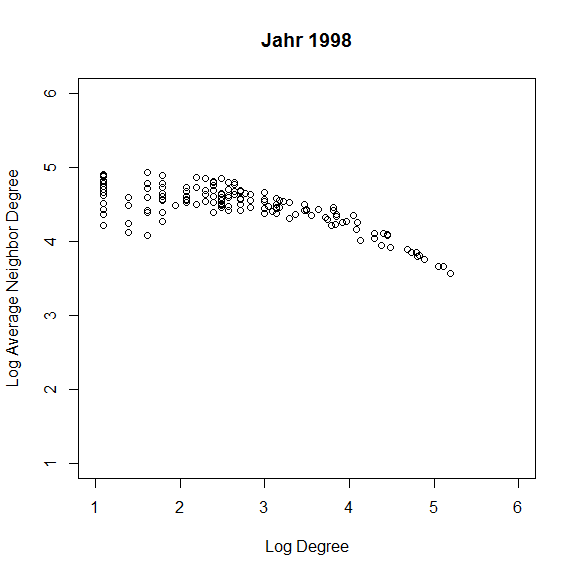
\includegraphics[width=0.60\textwidth]{Grafiken/and.png}
	\caption{Average nearest Neighbor Degree am Beispiel von 1998}
	\label{fig:and}
\end{figure}

Interessante Einblicke in die Zusammenhänge innerhalb eines Netzwerkes lassen sich auch generieren, indem man den Degree eines Knoten mit dem seiner Nachbarn vergleicht. Zwei Netzwerke mit gleicher Degree-Verteilung können dennoch unterschiedliche Strukturen besitzen, falls sich die Knoten der Netzwerke darin unterscheiden, mit welchen anderen Knoten sie sich bevorzugt verbinden. Hierzu betrachten wir Abbildung \ref{fig:and}. Hier ist das Jahr 1998 exemplarisch ausgewählt. Dem logarithmierten Knoten Degree auf der X-Achse ist der logarithmierte durchschnittliche Degree der Nachbarn auf der Y-Achse gegenübergestellt. Man erkennt, dass sich Knoten mit geringerem Degree tendenziell eher mit Knoten mit hohen Degree verbinden als mit Knoten, die selbst einen hohen Degree besitzen. Zentrale Akteure des Netzwerkes handeln also eher mit kleineren Akteuren des Netzwerkes als mit anderen zentralen Akteuren.


\section{Handelswerte}


Betrachtet man die Gewichte der Kanten, in diesem Fall die monetären Handelswerte, so fällt einem ein deutliches Ungleichgewicht auf. Wie Abbildung \ref{fig:ts_value} zeigt, ist die Summe der 1\% teuersten Waffenhandel über alle Jahre hinweg ähnlich der Summe der 99\% billigsten. Einige wenige große Waffentransaktionen wiegen also alle restlichen in ihrem monetären Gewicht auf. 
\begin{figure}[ht]
	\centering
		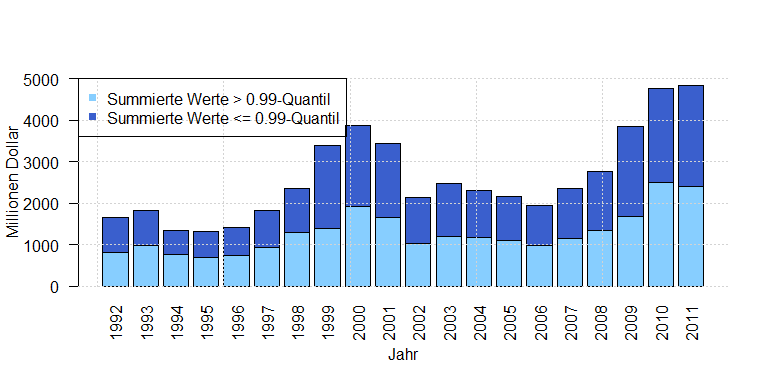
\includegraphics[width=0.7\textwidth]{Grafiken/ts_value.png}
	\caption{Vergleich der 1\% teuersten Waffenkäufe mit den 99\% billigsten in den Jahren 1992-2011}
	\label{fig:ts_value}
\end{figure}

\section{Top-Akteure}
\label{sec:top-akteure}
In Abschnitt \ref{sec:degree} wurde anhand der Degree-Verteilungen gezeigt, dass der Kleinwaffenhandel von einigen wenigen Nationen dominiert wird, die sich deutlich von der großen Masse der restlichen Akteure abheben. Diese sollen in diesem Abschnitt ermittelt werden. Hierzu werden in Tabelle \ref{tab:tops1} diejenigen Nationen aufgelistet, die über den Zeitraum von 20 Jahren das größte Import- und Exportvolumen, gemessen am Geldwert der gehandelten Waffen, aufweisen. 

\begin{table}[ht]

\centering

\begin{minipage}[t]{0.48\textwidth}
\footnotesize
\begin{tabular}{rlr}
  \hline
 Platz & Land & Exportvol. [Mrd.]\\ 
  \hline
1 & USA & 9.2\\ 
  2 & Italy & 7.9 \\ 
  3 & Germany & 4.6 \\ 
  4 & Brazil & 3.7 \\ 
  5 & Austria & 2.7 \\ 
  6 & United Kingdom & 2 \\ 
  7 & Belgium & 1.8 \\ 
  8 & Switzerland & 1.5 \\ 
  9 & Russia & 1.4 \\ 
  10 & Czech Republic & 1.4 \\ 
   \hline
	\end{tabular}
	\end{minipage}	
\hfill	
\begin{minipage}[t]{0.48\textwidth}	
\footnotesize
\begin{tabular}{rlr}
  \hline
 Platz & Land & Importvol. [Mrd.]\\ 
  \hline
1 & USA & 16\\ 
  2 & Germany & 2.3\\ 
  3 & France & 2.3\\ 
  4 & Canada & 1.9 \\ 
  5 & United Kingdom & 1.8\\  
  6 & Saudi Arabia & 1.7\\ 
  7 & Belgium & 1.2\\ 
  8 & Spain & 1.2\\ 
  9 & Australia & 1.2\\ 
  10 & Turkey & 1\\ 
   \hline
\end{tabular}
\end{minipage}
\caption{Summierte Handelswerte der Top-Importeure und Top-Exporteure des Netzwerkes von 1992 bis 2011}
\label{tab:tops1}
\end{table}


Es ist ersichtlich, dass die Vereinigten Staaten von Amerika mit 9.2 Milliarden Dollar am meisten Waffen exportieren. Italien steht mit 7.9 Milliarden Dollar Exportvolumen an zweiter Stelle. Deutschland exportiert mit 4.6 Milliarden Dollar gehandelten Waffen am dritt meisten. Auf dem vierten und fünften Platz folgen die Länder Brasilien und Österreich. Ab dem sechsten Platz erkennt man nur noch unwesentliche Verringerungen des Exportvolumens im Bereich von zwei bis eine Milliarden Dollar. Hierin befinden sich Nationen wie Großbritannien, Belgien, die Schweiz, Russland und die tschechische Republik. 

		
Auch bei den Importen steht die USA an erster Stelle. Die Nation gibt mit 16 Milliarden Dollar mehr für den Import von Kleinwaffen aus als die neun nachfolgenden Länder zusammen. Deutschland und Frankreich teilen sich mit 2.3 Milliarden Dollar Importvolumen den zweiten Platz. Auf der vierten Stelle befindet sich Kanada mit einem Importvolumen von circa 2 Milliarden Dollar. Großbritannien verwendet 1.8 Milliarden Dollar, um Waffen zu exportieren, und Saudi Arabien 1.7 Milliarden Dollar. Auf dem siebten, achten, neunten und zehnten Platz sehen wir vergleichbare Exportausgaben von circa 1.2 bis 1 Milliarde Dollar. Dies sind die Länder Belgien, Spanien, Australien und Türkei.

\begin{figure}[h]
\centering
	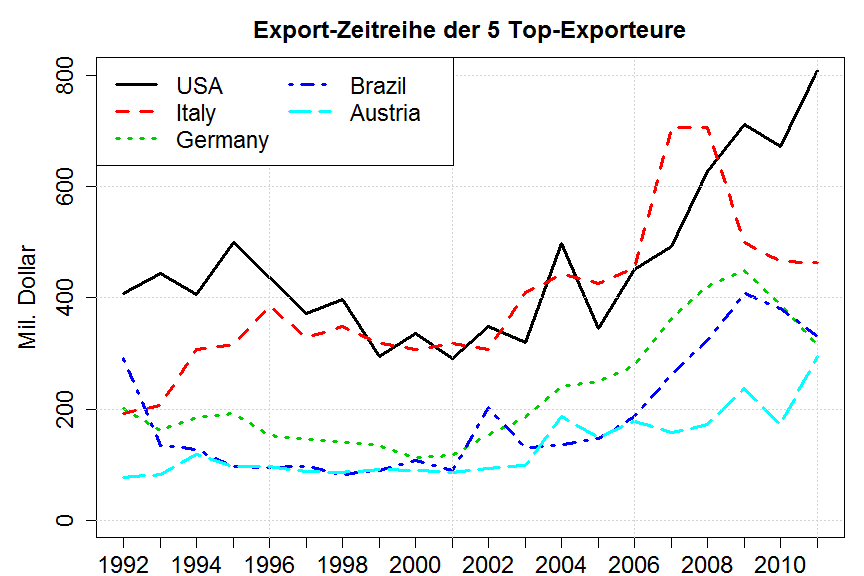
\includegraphics[width=0.65\textwidth]{Grafiken/ts_topsexp.png}
	\caption{Zeitreihen der jährlichen Handelswerte der Top-Exporteure von 1992 bis 2011}
	\label{fig:ts_tops1}
\end{figure}




Anschließend interessiert, ob sich die Handelsvolumen der Top-Exporteure und Importeure über die Jahre verändert. Hierfür betrachten wir für die Exporte die Abbildung \ref{fig:ts_tops1}.
In dieser Grafik sind die Handelsvolumen in Millionen US Dollar der fünf Top-Exporteure über den Zeitraum 1992 bis 2011 dargestellt. Die USA ist in fast allen Jahren der Waffenexporteur mit den höchsten monetären Volumen. Sie wird nur in wenigen Jahren von Italien übertroffen. Deutschland, Brasilien und Österreich exportieren in allen Jahren deutlich weniger Waffenwert als die USA. Auffällig ist ein relativ konstanter Verlauf der Zeitreihen im Zeitraum von 1992 bis circa 2001, während danach bei allen Ländern ein kräftiger Anstieg der Handelswerte feststellbar ist. Deutschland, Brasilien und vor allem Italien zeigen allerdings ab circa 2008 wiederum einen abfallenden Trend.

\begin{figure}[h]
\centering
	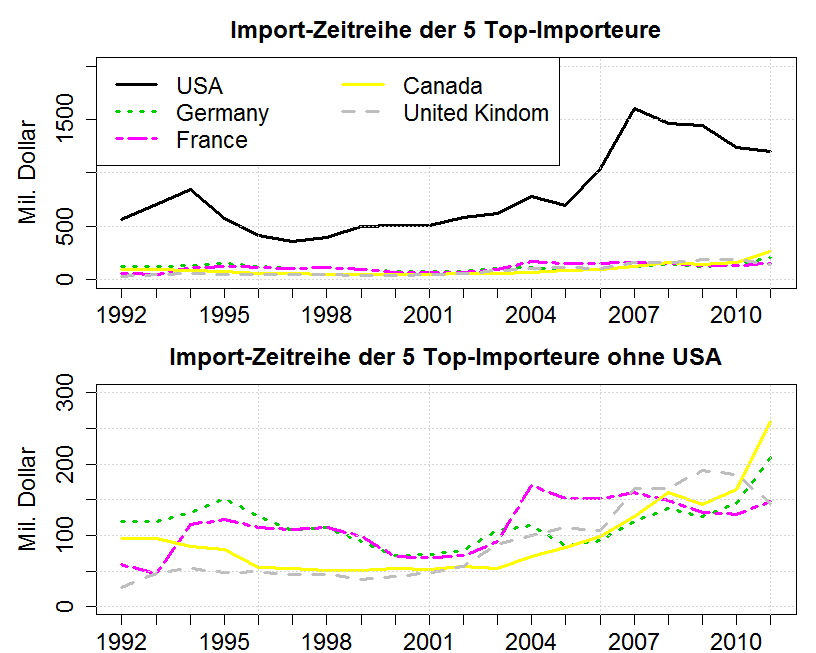
\includegraphics[width=0.65\textwidth]{Grafiken/ts_topsimp.png}
	\caption{Zeitreihen der jährlichen Handelswerte der Top-Importeure von 1992 bis 2011}
	\label{fig:ts_tops2}
\end{figure}

Die beiden Grafiken aus Abbildung \ref{fig:ts_tops2} zeigen die Handelsvolumen der Top-Importeure. Die USA ist hier unangefochten an der Spitze. Sie importiert Kleinwaffen im Wert zwischen circa 400 und 1600 Millionen US Dollar pro Jahr, während die restlichen Akteure höchstens Kleinwaffen im Wert von circa 250 Millionen Dollar pro Jahr einführen. Ähnlich wie bei den Exportzeitreihen ist auch hier ein relativ konstanter Verlauf bis circa 2001 zu beobachten, während die Ausgaben in den nachfolgenden Jahren kontinuierlich ansteigen. Die USA verringert ihre Importausgaben ab dem Jahr 2007 jedoch wieder deutlich. 

Bei den Top Akteuren des Waffenhandels handelt es sich also größtenteils um westliche Industrienationen. Diese bestimmen durch Wirtschaftskraft und großen Handelsvolumen sowohl den Export als auch den Import von Klein- und Leichtwaffen. Interessanter Weise bekommt man ein anderes Bild, wenn man die Handelswerte mit einem Maß der Wirtschaftskraft der Länder, hier dem Bruttoinlandsprodukt pro Kopf, skaliert. In Tabelle \ref{tab:tops2} sind diejenigen Länder aufgeführt, die relativ zu ihrem Bruttoinlandsprodukt pro Kopf im Zeitraum von 1992 bis 2011 am meisten Geld für den Import beziehungsweise den Export von kleinen und leichten Waffen ausgegeben haben.

	\begin{table}[ht]

\centering

\begin{minipage}[t]{0.45\textwidth}
\footnotesize
\centering
\begin{tabular}{rlr}
  \hline
 Platz & Land & Exportvol. / BIP pro Kopf\\ 
  \hline
1 & China & 114735 \\
2 & Brazil & 53225 \\
3 & Italy & 48862 \\
4 & Spain & 40822 \\
5 & Germany & 38039 \\ 
6 & Turkey & 36174 \\
7 & South Korea & 29131 \\
8 & United States & 26539 \\
9 & India & 24615 \\
10 & Austria & 23149 \\
   \hline
	\end{tabular}
	\end{minipage}	
\hfill	
\begin{minipage}[t]{0.45\textwidth}	
\centering
\footnotesize
\begin{tabular}{rlr}
  \hline
 Platz & Land & Importvol. / BIP pro Kopf\\ 
  \hline
1 &Tanzania &54562 \\
2 &Thailand &49636\\
3 &India &32416\\
4 &Pakistan &30290\\
5 &South Korea &27208\\
6 &China &25402\\
7 &Indonesia &24268\\
8 &Kenya &22907\\
9 &Malaysia &22330\\
10 &Burkina Faso &22183\\
   \hline
\end{tabular}
\end{minipage}
\caption{Summierte Handelswerte der Top-Exporteure und Top-Importeure relativ zum BIP pro Kopf des Netzwerkes von 1992 bis 2011}
\label{tab:tops2}
\end{table} 
Bei den Exporten sind immer noch die westlichen Industrienationen unter den zehn führenden Ländern am häufigsten vertreten. Auffallend ist, dass die zuvor deutlich dominierenden Vereinigten Staaten von Amerika nur noch auf dem achten Platz liegen. Gemessen an der eigenen Wirtschaftskraft exportiert China nun am meisten Waffen. Neu unter den zehn Führenden sind mit Indien und Süd Korea auch zwei wirtschaftsstarke asiatische Länder.
Im Gegensatz hierzu steht die Tabelle mit den zehn stärksten Importeuren von kleinen und leichten Waffen im Vergleich zu ihrer Wirtschaftskraft. Hier nehmen nun vor allem asiatische und afrikanische Entwicklungsländer die vorderen Plätze ein. Alle westlichen Industrienationen hingegen tauchen in den zehn vorderen Plätzen nicht mehr auf. Führend sind hier die Länder Tanzania, Thailand, Indien, Pakistan und Süd Korea.

Eine andere Methode, um zentrale Akteure des Netzwerkes zu identifizieren, ist sich die Degree-Sequenz der Netzwerkknoten zu betrachten. Welche Knoten (Länder) besitzen sowohl einen hohen In-Degree als auch einen hohen Out-Degree und können demnach als zentrale Akteure des Handelsnetzwerkes identifiziert werden?
\begin{figure}[h]
	\centering
		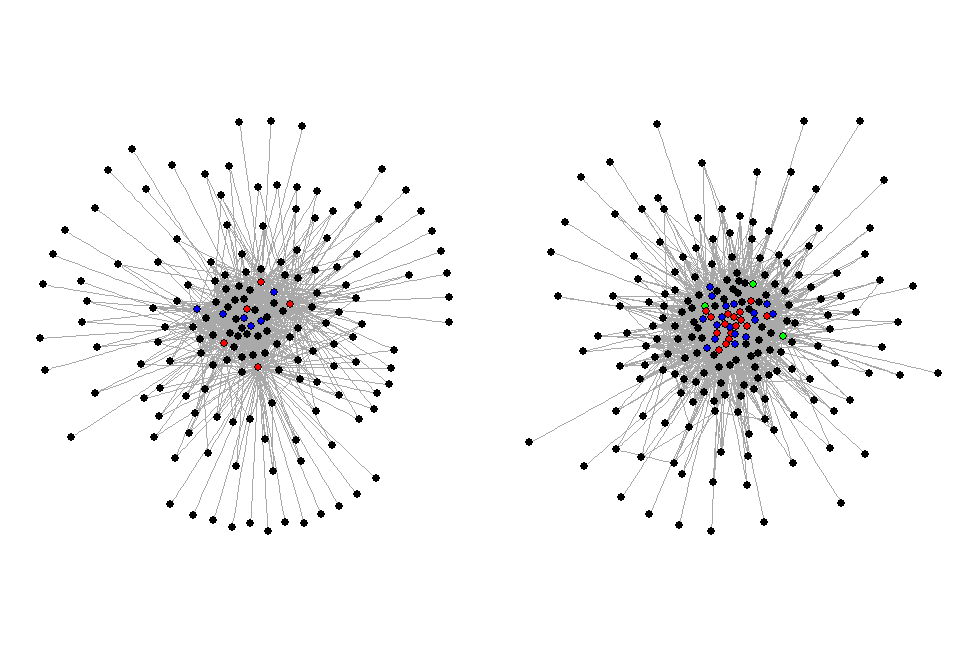
\includegraphics[width=0.90\textwidth]{Grafiken/ts_network.png}
	\caption{Visualisierung des Netzwerkes 1992 (l.) und 2011(r)}
	\label{fig:ts_network}
\end{figure}

Abbildung \ref{fig:ts_network} zeigt hierzu das gesamte Netzwerk in den Jahren 1992 und 2011. Jeder Punkt stellt ein am Waffenhandel beteiligtes Land dar. Ein Pfeil zwischen den beiden Ländern symbolisiert einen Handel. Länder mit einem In-Degree von größer als 30, die also aus mindestens 30 anderen Ländern Waffen beziehen, sind grün. Länder mit einem Out-Degree von größer als 30, die also an mindestens 30 andere Länder Waffen liefern, sind blau. Akteure, die beide Bedingungen erfüllen, sind rot eingefärbt. Übereinstimmend mit unseren einleitenden deskriptiven Analysen scheint das Netzwerk aus dem Jahr 2011 auf den ersten Blick größer und dichter zu sein als das Netzwerk im Jahr 1992. Auch die Anzahl der farblich markierten Knoten ist im Jahr 2011 deutlich größer als im Jahr 1992. Man erkennt also, dass die Anzahl der "`großen Akteure"' auf dem Kleinwaffenmarkt, gemessen an der Anzahl ihrer Importe und Exporte, über die Zeit deutlich zugenommen hat. In Tabelle \ref{tab:ZentrAkt} werden die rot markierten Knoten für beide Jahre aufgelistet. 


\begin{table}[h]
\centering
\footnotesize
\begin{minipage}[t]{0.48\textwidth}

\begin{center}
1992
\end{center}

\begin{tabular}{rlr}
  \hline
 Land 											& In-Degree & Out-Degree\\ 
  \hline
 Switzerland 								& 32				& 76\\ 
 USA 	& 43				& 105\\ 
 Germany & 47				& 118\\ 
 Spain 											& 36				& 62\\ 
 Sweden 										& 38 				& 33\\ 
   \hline

\end{tabular}
\end{minipage}
\hfill	
\begin{minipage}[t]{0.48\textwidth}

\begin{center}
2011
\end{center}

\begin{tabular}{rlr}
  \hline
 Land 						& In-Degree & Out-Degree\\ 
  \hline
 Switzerland 			& 41				& 103\\ 
 USA					 		& 63				& 145\\ 
 Finland 					& 34				& 70\\ 
 Italy 						& 39 				& 114\\ 
 France						& 41				& 82\\ 
 Poland						& 32				& 34\\
 Czech Rep.		& 37				& 105\\
 Germany					& 50				& 115\\
 UK		& 44				& 95\\
 Norway						& 32				& 39\\
 Spain  					& 37				& 91\\
 Canada						& 49				& 78\\
 Austria					& 41				& 108\\
 South Africa			& 34				& 32\\
 Belgium					& 31				& 64\\
 Australia				& 39				& 51\\
   \hline

\end{tabular}
\end{minipage}
\caption{Zentrale Akteure des Netzwerkes  1992 und 2011} 
\label{tab:ZentrAkt}
	\end{table}





\newpage
\section{Visualisierungen}



In diesem Abschnitt wird versucht, durch verschiedene Visualisierungen des Netzwerkes einen Überblick über mögliche Strukturen und Zusammenhänge des Kleinwaffenhandels zu erhalten. Da das Netzwerk recht groß ist, erzielt eine einfache Abbildung aller Knoten und Kanten, wie in Abbildung \ref{fig:ts_network} geschehen, ein nicht zufriedenstellendes Ergebnis. Ein möglicher Ansatz, um die Übersichtlichkeit der Visualisierung des Netzwerkes zu verbessern, ist es daher, die Knoten in Gruppen einzuteilen. Eine naheliegende Kategorisierung von Ländern sind die Kontinente, auf denen sie sich befinden. Diese Einteilung geschieht mit Hilfe des R-Pakets \emph{countrycode} \citep{countrycode}. Mit Hilfe der im Datensatz gegeben Correlates of War Country Codes und der kontinentalen Zuordnungen der Vereinten Nationen (UNO) weist dieses Softwarepaket jedem Land einen Kontinent zu. 34 der im Datensatz vorkommenden Länder sind sogenannte Sonderverwaltungszonen und werden daher keinem Kontinent zugeordnet. Beispiele hierfür sind Französisch Guyana, Hong Kong und die Falkland Inseln. Eine vollständige Liste aller Länder und ihrer Zuweisung eines Kontinentes findet sich im elektronischem Anhang dieser Arbeit.
Aus dieser Kategorisierung der Knoten resultiert die Grafik \ref{fig:cont}. 

In der Grafik ist die Größe der Knoten jeweils proportional zum Degree (In-Degree + Out-Degree), also der Anzahl der Handelsaktivitäten eines Knotens, gewählt. Die Breite der Kanten wiederum ist proportional zum monetären Wert der Handelsströme zwischen zwei Kontinenten gewählt. Die Positionierung der Knoten wurde zur besseren Vergleichbarkeit der Jahre untereinander fixiert.
In Abbildung \ref{fig:cont} erkennt man, dass Europa durchgängig mit dem größten Kreis markiert ist, also an mehr Handelsaktionen beteiligt ist als die anderen Kontinente. Die Dicke der Kanten und damit der zwischen den Kontinenten gehandelte monetäre Wert variiert stark zwischen den Jahren. Hier ist kein gleichbleibendes Muster zu erkennen.

\begin{figure}[ht]
\centering
\animategraphics[scale=0.7, controls]{1}{Grafiken/Cont_Ani/cont}{1}{20}
\caption{Handelsströme zwischen den Kontinenten von 1992 bis 2011}
\label{fig:cont}
\end{figure}


\chapter{Exponential Random Graph Model}
 Wie bereits in der Einleitung erläutert, stellt die Abhängigkeitsstruktur der Beobachtungen in einem Netzwerk besondere Ansprüche an die statistische Modellierung eines Netzwerkes. Aus der deskriptiven Analyse unseres Datensatzes geht außerdem hervor, dass die Kantenbildung zwischen zwei Knoten in unserem Netzwerk nicht nur von der Struktur des restlichen Netzwerkes sondern auch von exogenen Kovariablen wie zum Beispiel der Wirtschaftskraft und der geografischen Lage eines Landes abhängt.

Üblicherweise verwendet man zur Modellierung von Netzwerken das \emph{Exponential Random Graph Model (ERGM)}, denn
\begin{quote}
"`The ERGM is a statistical model that can be used to estimate the effects of covariates on the ties in a network while simultaneously estimating parameters that provide a precise and parismonious description of the forms of dependence that can exist in relational data."' \citep{cranmer2011inferential}
\end{quote}
Das ERGM kann also sowohl den Einfluss exogener Kovariablen als auch den strukturellen endogenen Einfluss eines Netzwerkes auf sich selbst modellieren. In den folgenden Abschnitten wird zunächst das Modell theoretisch erklärt, um es danach auf den Datensatz zum Handel mit kleinen und leichten Waffen anzuwenden. Die Definition des Modells in Abschnitt \ref{sec:defmod} folgt im wesentlichen dem Artikel von \citet{hunter2008ergm}. Die darauf folgenden Abschnitte \ref{sec:simzuf} und \ref{sec:modpar} wurden aus den Kapiteln 12.2 und 12.3 des Buches von \citet{lkr12} erarbeitet.
%Abschnitt \ref{sec:defmod} folgt \citep{hunter2008ergm}.
%Abschnitt \ref{sec:simzuf} folgt \citep[Kapitel 12.2]{lkr12}.
%Abschnitt \ref{sec:modpar} folgt \citep[Kapitel 12.3]{lkr12}.

\section{Definition des Modells}
\label{sec:defmod}
Vorab einige notwendige Notation:

Sei $X$ eine matrixwertige Zufallsvariable und repräsentiere die Nachbarschaftsmatrix eines Netzwerkes. $\mathcal{X}$ soll die Menge aller möglichen Nachbarschaftsmatritzen von binären Netzwerken mit fester Knotenanzahl $N_V$ darstellen, die keine Schleifen oder multiple Kanten enthalten. Daher ist $\mathcal{X}$ die Menge aller $N_V \times N_V$ Matritzen, deren Einträge entweder Eins oder Null sind und die auf ihrer Diagonalen nur Nuller besitzen. Das $ij$-te Element von $X$ repräsentiert eine Kante zwischen Knoten $i$ und $j$. Bei einem ungerichteten Netzwerk ist $X$ eine symmetrische Matrix. Bei einem gerichteten Netzwerk kann sich hingegen der Eintrag an der Stelle $ij$ von dem an der Stelle $ji$ unterscheiden.

Die Wahrscheinlichkeitsverteilung der matrixwertigen Zufallsvariable $X$ lässt sich nun in folgender Form ausdrücken:
\begin{equation}
P_{\theta, \mathcal{X}}(X = x) = \frac{exp\left\{\theta^T g(x)\right\}}{\kappa(\theta, \mathcal{X, Y})}
\label{eq:ergm}
\end{equation}
mit

\begin{itemize}
	\item $x \in \mathcal{X}$
	\item $\theta \in \Omega \subset \mathbb{R}^q$ ... Vektor der Modellparameter.
	\item $g(x)$ ... q-Vektor aus Statistiken basierend auf der Nachbarschaftsmatrix $X$.
\end{itemize}
Ersetzt man in Gleichung \ref{eq:ergm} $g(x)$ durch $g(x,Y)$, so ermöglicht man die Aufnahme von zusätzlichen exogenen Informationen $Y$ über das Netzwerk (siehe Kapitel \ref{sec:exkov}). $\kappa(\theta, \mathcal{X}) = \sum_{x \in \mathcal{X}}{exp\left\{\theta^T g(x)\right\}}$ ist ein Normalisierungsfaktor, der sicherstellt, dass sich bei der Gleichung \ref{eq:ergm} eine Wahrscheinlichkeitsverteilung mit Wertebereich $[0,1]$ ergibt. Die genaue Berechnung von $\kappa(\theta, \mathcal{X})$ ist problematisch, da die Summe über alle möglichen Ausprägungen der Zufallsvariable $\mathcal{X}$ summiert. Da aber bereits bei $n$ Knoten $2^{n(n-1)}$ verschiedene Netzwerke denkbar sind, erhält man schnell eine unvorstellbar große Anzahl an möglichen Netzwerken, die den Umgang mit  $\kappa(\theta, \mathcal{X})$ zum entscheidenden Problem dieses Modells werden lassen. Eine analytische Lösung des Modells ist hierdurch oft unmöglich. Es werden Methoden benötigt, um durch simulationgestützte Verfahren geeignete Schätzer entwickeln zu können. Hiermit beschäftigen sich die nächsten beiden Kapitel.

\subsection{Simulation von Zufallsgraphen}
\label{sec:simzuf}
Die Simulation von Zufallsgraphen aus einer Zielverteilung $P_\theta(x)$ basiert auf dem Makrov Chain Monte Carlo (MCMC) Algorithmus. Hierbei beginnt man mit einem beliebigen Netzwerk mit fester Knotenzahl $N_V$. Nun sucht man sich ein zufälliges Knotenpaar und fügt zwischen ihnen eine Verbindung hinzu beziehungsweise entfernt eine bereits bestehende Verbindung. Besitzt der so erhaltene Graph nun eine höhere Wahrscheinlichkeit als der vorherige, so wird er akzeptiert. Besitzt der neue Graph eine geringere Wahrscheinlichkeit, so wird er mit einer Wahrscheinlichkeit akzeptiert, die proportional zum Verhältnis der Wahrscheinlichkeiten von altem und neuem Graph ist. Nach ausreichend großer Anzahl von Iterationen erhält man ein zufälliges Netzwerk, das als Ziehung aus der Zielverteilung $P_\theta(x)$ angesehen werden kann. Alle vorherigen Ziehungen werden verworfen und als \emph{Burn In} bezeichnet. Der Burn In wird benötigt, damit der Algorithmus den beliebig gewählten Anfangszustand "`vergessen"' kann. Bei ausreichend großem Burn In ist das gezogene Netzwerk unabhängig vom Startpunkt und jedes der nach ihm gezogenen Netzwerke entspringt ebenfalls der Zielverteilung.
Genauer gesagt wird ein Metropolis Algorithmus verwendet. Man erstellt hierbei eine Sequenz von Graphen $X^{(0)}, X^{(1)}, ..., X^{(M-1)}, X^{(M)}$. Im $m$-ten Iterationsschritt wird hierbei folgendermaßen vorgegangen:

\begin{enumerate}
	\item Aus dem aktuellen Graphen $x^{(m-1)}$ wird ein zufälliges Knotenpaar $i,j$ ($i,j \in 1, ...,N_V$) ausgewählt.
	\item Der vorgeschlagene Graph $x^* = x^{(m-1)}$ bis auf $x_{ij}^{*} = 1 - x_{ij}^{(m-1)}$.
	\item Der vorgeschlagene Graph wird mit der Wahrscheinlichkeit $min\{1, \frac{P_{\theta}(x^*)}{P_{\theta}(x^{m-1})}\}$ akzeptiert.
	\item Bei Akzeptanz entspricht der neue Graph $x^m = x^*$ und sonst $x^m = x^{m-1}$.
\end{enumerate}
Hierbei ist für das Verhältnis von $\frac{P_{\theta}(x^*)}{P_{\theta}(x^{m-1})}$ die Berechnung der Change-Statistiken ausreichend, denn

\begin{align*}
log\{\frac{P_{\theta}(x^*)}{P_{\theta}(x^{m-1})}\} &= log\{P(X_{ij} = 1-x_{ij}^{m-1}|X_{-ij}=x_{ij}^{m-1}\} \\
																										&= \theta_1(z_1(x^*) - z_1(x^{m-1})) + \theta_2(z_2(x^*) - z_2(x^{m-1}))\\   																									& + ... + \theta_p(z_p(x^*) - z_p(x^{m-1})).
\end{align*}

Der rechnerische Aufwand dieser Methode kann optimiert werden, indem man zum Beispiel größere Update-Schritte oder Update-Schritte mit ungleichen Gewichten zulässt.

Will man mehrere Graphen aus der selben Verteilung ziehen, so kann die gleiche Kette verwendet werden. Allerdings sind zwei direkt nacheinander beobachtete Graphen einer Kette natürlich stark korreliert. Daher lässt man zwischen den beobachteten Graphen jeweils $k$ Iterationen aus. Den Wert von $k$ nennt man \emph{Thinning}. Die Autokorrelation zwischen den gezogenen Graphen sollte durch ein möglichst großes $k$ gering gehalten werden.

\subsection{Schätzung der Modell-Parameter}
\label{sec:modpar}
Ziel der Schätzung der Parameter ist es, die Verteilung der Statistiken der simulierten Netzwerke über den Statistiken des beobachteten Netzwerkes zu zentrieren, so dass
\begin{equation}
	E_\theta(z(X)) - z(x_{obs}) = 0.
	\label{eq:1}
\end{equation}
Das Auflösen von Gleichung \ref{eq:1} liefert die Parameterwerte $\theta$, die die beobachteten Daten $x_{obs}$ am besten beschreiben.
Analog hierzu funktioniert die Maximum Likelihood Theorie. Hier wird derjenige Parametervektor $\theta$ gesucht, der die Wahrscheinlichkeit $P_\theta(x_{obs})$ maximiert. Dieses Vorgehen liefert den gleichen $\theta$-Vektor wie die Lösung von Gleichung \ref{eq:1}, denn die partielle Ableitung nach $\theta$ liefert
\begin{align*}
\frac{\partial}{\partial \theta} log(P_\theta(x_{obs})) &= z(x_{obs}) - \frac{\partial}{\partial \theta} log\{\sum_{x \in X}{exp(\theta_1z_1(x)+ ... + \theta_pz_p(x))}\}\\
&=z(x_{obs}) - \sum_{x \in X}{z(x)P_\theta(x)},
\end{align*}
was Gleichung \ref{eq:1} entspricht. 

Eine analytische Lösung dieser Gleichung ist auf Grund der großen Anzahl an möglichen Netzwerken nicht möglich. Im Prinzip funktioniert die Lösung der Gleichung deshalb durch einfaches Ausprobieren. Das bedeutet, man wählt einen beliebigen Parametervektor, simuliert mit diesem auf oben erklärte Art und Weise eine große Anzahl an Graphen und überprüft im Anschluss, ob Gleichung \ref{eq:1} erfüllt ist. Dieses Vorgehen ist aber natürlich vom Rechenaufwand ineffizient. Eine Möglichkeit zur effizienteren Implementierung dieses Vorgehens bietet das \emph{Importance Sampling} nach Geyer-Thompson, welches im \texttt{statnet} Paket \citep{pack:statnet} in R  \citep{R} standardmäßig verwendet wird. Der Geyer-Thompson Algorithmus zieht eine große Stichprobe von Graphen für einen vorläufigen Parametervektor $\widetilde{\theta}$. Diese Stichprobe wird nun als repräsentativ für alle Graphen angesehen. Die Stichprobe wird immer weiter verwendet, selbst wenn sich der Parametervektor im Laufe des Algorithmus verändert. Um zu berücksichtigen, dass es sich nur um eine Stichprobe und keine vollständige Sammlung aller möglichen Graphen handelt, muss bei der Berechnung von $\bar{z}_\theta$ ein gewichteter Durchschnitt der Statistiken verwendet werden. Falls die Stichprobe aus der Verteilung $P_\theta(x)$ generiert wurde, ist der Stichprobendurchschnitt $\bar{f}_\theta = w^1 f(x^1) + w^2 f(x^2) + ... + w^M f(x^M)$ der Funktion $f$ mit den Gewichten $w^{(m)} = \frac{e^{(\theta_1-\widetilde{\theta}_1)z_1(x^{(m)})+...+(\theta_p-\widetilde{\theta}_p)z_p(x^{(m)})}}{\sum_{k=1}^{M}{e^{(\theta_1-\widetilde{\theta}_1)z_1(x^{(k)})+...+(\theta_p-\widetilde{\theta}_p)z_p(x^{(k)})}}}$ 
eine gute Approximation für den echten Erwartungswert $E_\theta(f(X))$, wenn M groß wird und $\widetilde{\theta}$ nahe am wahren $\theta$ liegt. Umso näher $\widetilde{\theta}$ und $\theta$ zusammen liegen, desto näher kommen die Gewichte dem Wert $\frac{1}{M}$. Falls $\theta$ und $\widetilde{\theta}$ jedoch weiter auseinander liegen, besitzen die Gewichte eine hohe Streuung und somit die Schätzung eine große Standartabweichung.
Um die Likelihood nun zu lösen, erzeugt man eine Sequenz von Parametern $\widetilde{\theta},\theta^{1}, \theta^{2},...,\theta^{G}$ mit Hilfe eines Verfahrens wie \emph{Newton-Raphson} oder \emph{Fisher Scoring}. Eine Aktualisierung der Sequenz erfolgt durch $\theta^{(g)} = \theta^{(g-1)} - {D(\theta^{(g-1)})}^{-1}\left\{\sum^{M}_{m = 1}{w^{(m)}z(x^{(m)})} - z(x_{obs})\right\}$. Da $\sum^{M}_{m = 1}{w^{(m)}z(x^{(m)})}$ eine Approximation von $E_\theta(z(X))$ ist, falls $\theta^{(g-1)}$ der wahre Parameter ist, ergibt sich dann $E_\theta(z(X)) - z(x_{obs}) = 0$ und $\theta^{(g)}$ bleibt unverändert zu $\theta^{(g-1)}$. Die Skalierungsmatrix $D(\theta)$ skaliert die Unterschiede zwischen den beobachteten und simulierten erwarteten Werten der Statistiken, da die Statistiken sich in ihrer Sensitivität gegenüber Parameteränderungen unterscheiden können und die Parameterwerte nicht nur ihre eigenen sondern auch fremde Statistiken beeinflussen können. $D$ ist die gewichtete Stichproben Kovarianzmatrix $\Sigma_m w^{(m)} z(x^{(m)}) z(x^{(m)})^T - \left[\Sigma_m w^{(m)} z(x^{(m)}\right] \left[\Sigma_m w^{(m)} z(x^{(m)}\right]^T$.
Typischer Weise startet man diesen Algorithmus einige Male und setzt den vorgeschlagenen Parameter $\widetilde{\theta}$ gleich $\theta^{(G)}$. Für diesen Algorithmus ist es sehr wichtig, dass man den Startpunkt $\widetilde{\theta}$ nicht zu weit entfernt vom richtigen ML-Schätzer wählt, was in der Praxis schwierig sein kann. Zusammengefasst lässt sich das Prinzip des Importance-Sampling schematisch folgendermaßen darstellen:

	\begin{enumerate}
		\item Ziehung einer großen Stichprobe von Graphen auf Basis eines vorläufigen Parametervektors $\tilde{\theta}$.
		\item Benutzung gewichteter Stichprobendurchschnitte der Statistiken.
		\item Erzeugen einer Sequenz von Parametern $\widetilde{\theta},\theta^{(1)}, \theta^{(2)},...,\theta^{(G)}$ durch \emph{Fisher Scoring}.
		\item Neustart mit $\theta^{(G)}$ als $\tilde{\theta}$.
	\end{enumerate}


\section{Endogene Statistiken}
Netzwerkdaten sind in der Regel relationale Daten. Das bedeutet, sie beschränken sich nicht lediglich auf Variablen die einzelne Akteure betreffen, sondern zeichnen sich viel mehr dadurch aus, dass sie Beziehungen zwischen ihnen abbilden. Die Knoten(Akteure) eines Netzwerkes können daher genauso wenig wie die sie verbindenden Kanten als unabhängig voneinander betrachtet werden. Sie hängen explizit vom Zustand des restlichen Netzwerkes ab. Diese Eigenschaft erschwert die richtige Spezifizierung und Schätzung eines Modells im Vergleich zur gewöhnlichen statistischen Inferenz \citep{handcock2008statnet}. 

Die Zielvariable in einem Exponential Random Graph Model ist die Existenz beziehungsweise Abwesenheit einer Kante. Als erklärende Kovariablen werden hierbei Statistiken verwendet, die aus Funktionen eben genau dieser Kanten hervorgehen. Man kann das Modell also in gewisser Weise als autoregressives Modell betrachten \citep{morris2008specification}. Welche Statistiken aufgenommen werden sollten, um ein gutes Modell zu erhalten, lässt sich nicht allgemeingültig beantworten. Abhängig von Struktur und Art des Netzwerkes sollten aus den im Folgenden vorgestellten Gruppen die jeweils passenden gewählt werden. Für eine (vollständige) Auflistung der im \texttt{ergm}-Paket \citep{pack:ergm} implementierten Statistiken verweise ich auf \citep{morris2008specification} und die entsprechende Hilfe Seite in R.

Die Basis eines jeden Modells sollte eine Statistik bilden, die die Grundwahrscheinlichkeit der Bildung einer Kante im Netzwerk wiedergibt. Üblicherweise verwendet man hierfür die Anzahl an Kanten, die im \texttt{ergm}-Paket durch die Statistiken \textit{edge} und \textit{density} implementiert sind und im Falle eines gerichteten Netzwerkes äquivalent sind. Zusätzlich können die Statistiken \textit{mutual} und \textit{asymmetric} verwendet werden, die die Anzahl an Knotenpaaren $i$,$j$ zählen, für die sowohl die Kante $(i,j)$ als auch die Kante $(j,i)$ besteht, beziehungsweise eben nur genau eine von beiden.

Die Degree-Verteilung, wie in Abschnitt \ref{sec:degree} beschrieben, lässt sich durch den Term \textit{degree(d)} im Modell berücksichtigen. Diese Statistik zählt alle Knoten im Netzwerk, die genau den Degree $d$ aufweisen. In einem gerichteten Netzwerk verwendet man \textit{idegree(d)} und \textit{odegree(d)} für In- und Out-Degree. Eine ähnliche Statistik ist \textit{kstar(k)}. Sie zählt die Anzahl an \emph{k-stars} im Netzwerk. Ein k-star ist definiert als ein Knoten, der zu $k$ anderen Knoten eine Kante besitzt. Anders als bei \textit{degree} kann hier ein Knoten mehr als einmal gezählt werden. Bei gerichteten Netzwerken verwendet man alternativ \textit{istar(k)} und \textit{ostar(k)}.

Gruppenbildungen und Transitivitätseigenschaften lassen sich bei gerichteten Netzwerken durch Statistiken wie \textit{ctriple, ttriple} oder \textit{transitive} erfassen. Diese führen aber bekannter Weise zur Degenerierung des modellierten Netzwerkes (siehe zum Beispiel \citep{morris2008specification, hunter2008ergm, handcock2008statnet}) und werden deshalb gerne durch alternative neuere Statistiken ersetzt, die im folgenden Abschnitt vorgestellt werden.

\section{Degeneration und alternative Modellierung}
\label{sec:degeneration}
In diesem Absatz gebe ich die Erklärungen zur Degeneration aus \citet{handcock2008statnet} wieder, falls nicht anders ausgewiesen.

Ein häufig auftretendes Problem des Exponential Random Graph Modells ist, dass das simulierte Modell degeneriert. Man spricht von einem degenerierten Modell, falls es einen Großteil seiner Wahrscheinlichkeitsmasse auf wenige extreme und unrealistische Netzwerkkonfigurationen wie zum Beispiel ein volles oder komplett leeres Netzwerk legt. Für eine genauere mathematische Erklärung verweise ich auf \citet{handcock2003assessing}. Ein degeneriertes Modell führt oft zur Divergenz des Schätzalgorithmus, wodurch der ML-Schätzer der Parameter im Modell nicht bestimmt werden kann. 
\begin{quote}
"`Degeneracy is an implication of network mis-spezifikation - not a short coming of the MCMC estimation procedure."'\citep{handcock2008statnet}
\end{quote}
Der Grund, dass einfache Zählstatistiken wie \textit{ttriple} oder \textit{ctriple} zur Degeneration eines Netzwerkes führen, ist, dass die Hinzunahme einer einzelnen Kante ihren Wert so stark verändern kann, dass der Einfluss des Parameterwerts auf das Netzwerk unrealistisch verstärkt wird. Das wird an einem einfachen Beispiel deutlich: Ein Knoten mit Degree vier besitzt sechs Two-Stars. Verbindet man ihn jedoch mit nur einem einzigen weiteren Knoten, so kommen bereits auf einen Schlag vier weitere Two-Stars hinzu. Hierfür gibt es in der neueren Netzwerkforschung eine empfohlene Lösungsstrategie: die Aufnahme von nicht linearen Einflüssen durch sogenannte \emph{Curved Exponential Family Models(CEFM)} \citep{hunter2007curved}.

Die Beschränkung auf lineare Effekte der Statistiken scheint intuitiv unrealistisch zu sein. Man denke sich ein Freundesnetzwerk. Zwei Akteure mit keinem oder einem guten Freund werden sich deutlicher voneinander unterscheiden als zwei Akteure mit 20 oder 21 guten Freunden. Der Einfluss der Veränderung der Degree-Statistik um eins sollte also mit der Höhe der Statistik abnehmen. Dies gewährleistet zum Beispiel die \textit{Geometrically Weighted Degree} (GWD) Statistik:
\begin{equation}
	u(x, \phi_s) = e^{\phi_s} \sum^{n-1}_{i=1}\left\{1-(1-e^{-\phi_s})^{i}\right\}D_i(x)
	\label{eq:GWD}
\end{equation}
$u(x,\phi_s)$ ist hierbei eine Funktion der Degreestatistiken $D_i(x)$ abhängig vom Parameter $\phi_s$.

Ähnliche Statistiken, die Stern und Dreiecks-Statistiken ersetzen können, sind die \textit{Geometrically Weighted Edgewise Shared Partners} (GWESP) und \textit{Geometrically Weighted Dyadic Shared Partners} (GWDSP) Statistiken $v$, $w$:
\begin{equation}
	v(x, \phi_t) = e^{\phi_t} \sum^{n-2}_{i=1}\left\{1-(1-e^{-\phi_t})^{i}\right\}EP_i(x)
	\label{eq:GWESP}
\end{equation}
\begin{equation}
	w(x, \phi_p) = e^{\phi_p} \sum^{n-2}_{i=1}\left\{1-(1-e^{-\phi_p})^{i}\right\}DP_i(x)
	\label{eq:GWDSP}
\end{equation}
$EP_i(x)$ zählt die Anzahl der Kanten in $x$, die genau $i$ gemeinsame Nachbarn haben. $DP_i(x)$ zählt die Anzahl der Knotenpaare $(k,l)$ in $x$, die genau $i$ gemeinsame Nachbarn haben unabhängig von $X_{kl}$.

Die Parameter $\phi_s, \phi_t$ und $\phi_p$ sind sogenannte Decay-Parameter und bestimmen den Grad, in dem der Effekt der Statistiken für größere Werte abnimmt. Umso größer $\phi$, desto langsamer ist die Abnahme des Effekts.
\section{Exogene Kovariablen}
\label{sec:exkov}
Ein weiterer möglicher Grund für die Degeneration eines Modells ist das Fehlen von exogenen Unterscheidungsmerkmalen. In einem ERGM, das nur mit endogenen Statistiken arbeitet, werden zunächst alle Knoten als gleich angenommen und dadurch bekommen alle strukturgleichen Netzwerke die gleiche Wahrscheinlichkeit zugewiesen. Eigenschaften einzelner Knoten oder Kanten werden hier also nicht weiter berücksichtigt. Im deskriptiven Teil dieser Arbeit wurde aber gezeigt, dass die Teilnahme am Waffenhandelsnetzwerk durchaus von Eigenschaften wie der Wirtschaftskraft oder der geographischen Lage eines Landes abhängig ist. Um also ein gutes Modell anzupassen, werden exogene Kovariablen benötigt, die Informationen über diese Eigenschaften liefern.
Bei der Analyse des SALW Datensatzes standen folgende exogene Kovariablen zur Verfügung:

\subsection{Polity Score}
Der verwendete Datensatz entspringt dem \emph{Polity IV Project}, welches vom \emph{Center for Systemic Peace} (CSP) \citep{polity} betrieben wird. Dieser Datensatz weißt jedem Land abhängig von seinem Demokratiestatus einen Wert zwischen $-10$ und $10$ zu. $-10$ kennzeichnet hierbei den schlechtest möglichen Wert, wobei $10$ für bestmögliche demokratische Standards steht. Verwendet wird eine gewichtete Nachbarschaftsmatrix, deren $ij$-ter Eintrag dem Unterschied im Demokratiescore zwischen Land $i$ und Land $j$ entspricht.

\subsection{Composite Index of National Capability}
Der \emph{Composite Index of National Capability} aus der neusten Version des \emph{National Material Capabilities Dataset}(Version 4.1)  \citep{CINC} ist ein Maß der nationalen Macht, dass vom Correlates of War Projekt erstellt wurde. Der Index berücksichtigt die Gesamtbevölkerungsanzahl, die Anzahl urbaner Bevölkerung, die Eisen- und Stahlproduktion, den Energieverbrauch sowie die Militärausgaben und Militärgröße eines Landes. Diese Daten liegen nur bis zum Jahr 2007 vor und dienen hier als Knotenattribut.

\subsection{Intra-State Conflicts}
Eine zusätzliche Kovariate in unserem Modell sammelt Informationen über internationale, zivile sowie ethnische Gewalt und Kriege. Die Daten kommen vom \emph{Major Episodes of Political Violance} Projekt \citep{conflict}, das wie auch das Polity IV Projekt von CSP bereitgestellt wird. Die Konflikte sind, abhängig von der Stärke ihrer Auswirkung auf die betroffene Bevölkerung, auf einer Skala von $1-10$ bewertet.

\subsection{GDP}
Zu guter Letzt verwenden wir auch das Bruttoinlandsprodukt der Länder als Knotenattribut. Die Daten entstammen dem \emph{Maddison Project}\citep{GDP}. 

\section{Geschätzte Modelle}

Nach den vorhergehenden theoretischen Überlegungen und einigem Ausprobieren ergibt sich ein Modell, dessen Output in Tabelle \ref{tab:model1} wiedergegeben ist. Aufgenommen wurden die beiden einfachen Statistiken \emph{edges} und \emph{mutual} und die in Abschnitt \ref{sec:degeneration} eingeführten Statistiken \emph{gwdegree}, \emph{gwesp} und \emph{gwdsp}. Alle zur Verfügung stehenden exogenen Kovariablen werden in das Modell mit aufgenommen. Zusätzlich beinhaltet das Modell die Kontinente der Länder als faktorielle Einflussgröße.

\begin{table}[ht]
	\centering
	\caption{Summary von Modell 1 im Jahr 1996}
		\begin{tabular}{l|l|l|l}
		
		\hline
		ergm-term 						   				  & Estimate      & Std.Error   & p-Value 				\\
		\hline
    edges                     				& -6.111e+00  &2.281e-01      & < 1e-04 *** \\
    mutual                   					&  2.120e+00  &9.507e-02      & < 1e-04  ***\\
    gwidegree                  				&  1.895e+00  &4.818e-01      & < 1e-04  ***\\
    gwodegree                     		& -1.311e+00  &3.307e-01      & < 1e-04  ***\\
    gwesp.fixed.0.2                   &  2.641e+00  &1.778e-01      & < 1e-04  ***\\
    gwdsp.fixed.0.2				    				& -5.686e-02  &6.008e-03      & < 1e-04  ***\\
    nodeicov.ext\_cinc         				&  3.071e+00  &1.291e+00      & 0.01740  *\\
    nodeocov.ext\_cinc         				& -5.967e+00  &1.361e+00      & < 1e-0  ***\\
    nodeicov.ext\_gdp          				&  3.479e-06  &2.099e-06      & 0.09749  .\\
    nodeocov.ext\_gdp          				&  4.392e-06  &1.586e-06      & 0.00562  **\\
    nodeicov.ext\_conflict     				&  2.310e-02  &1.704e-02      & 0.17530  \\
    nodeocov.ext\_conflict     				& -1.398e-01  &2.763e-02      & < 1e-04  ***\\
    nodeifactor.Continent.America     &  6.645e-02  &6.799e-02      & 0.32839  \\
		nodeifactor.Continent.Asien     	&  9.525e-02  &6.473e-02      & 0.14116  \\
		nodeifactor.Continent.Europe     	&  5.353e-03  &7.312e-02      & 0.94164  \\
		nodeifactor.Continent.Oceania     & -2.323e-02  &1.136e-01      & 0.83795  \\
    nodeofactor.Continent.America     &  2.055e-01  &6.589e-02      & 0.00182  **\\
		nodeofactor.Continent.Asien     	&  1.494e-01  &6.452e-02      & 0.02055  *\\
		nodeofactor.Continent.Europe     	&  8.579e-01  &7.226e-02      & < 1e-04  ***\\
		nodeofactor.Continent.Oceania     &  2.311e-01  &9.602e-02      & 0.01611  *\\
		absdiff.ext\_polity            		& -9.360e-03  &3.249e-03      & 0.00397 **\\
		\hline
		\end{tabular}
		\label{tab:model1}
\end{table}
In Tabelle \ref{tab:model1} sind die Ergebnisse der Schätzung von Modell 1 im Jahr 1996 angegeben. Nahezu alle aufgenommenen Statistiken erweisen sich als signifikant. Lediglich der Faktor Kontinent für den Export und die Kovariable Conflict für den Import haben keinen signifikanten Einfluss auf den Handel mit kleinen und leichten Waffen (p-Wert > 0.1).

\subsection{Interpretation der Parameter}
Zur anschaulichen Interpretation der Parameterwerte stelle man sich zwei Netzwerke $X^{(1)}$ und $X^{(2)}$ vor, die in allen Statistiken gleich sind, bis auf in der Statistik $g_i(X)$ mit
$$\delta_i(X) = g_i(X^{(1)}) - g_i(X^{(2)}).$$


Für eine einfache Interpretation der Modellparameter lässt sich Modellgleichung \ref{eq:ergm} nun umschreiben zu 
\begin{equation}
\frac{P(X^{(1)})}{P(X^{(2)})} = exp(\theta_i \delta_i(X))
	\label{eq:interpretation}
\end{equation}
Das Verhältnis der Wahrscheinlichkeiten der beiden Netzwerke auf der linken Seite von Gleichung \ref{eq:interpretation} hängt nun also nur von dem Unterschied der beiden Netzwerke in der Statistik $g_i$ und dem dazugehörigen Parameter $\theta_i$ ab. Nehmen wir nun an, die Statistik $g_i$ sei im Netwzerk $X^{(1)}$ größer als im Netzwerk $X^{(2)}$, so ist $\delta_i(X) > 0$ und es ergibt sich eine einfache Interpretation des Parameters $\theta_i$:
	\begin{itemize}
		\item Ist $\theta_i > 0$, so ist $X^{(1)}$ plausibler als $X^{(2)}$.
		\item Ist $\theta_i = 0$, so sind sie gleich plausibel.
		\item Ist $\theta_i < 0$, so ist $X^{(2)}$ plausibler als $X^{(1)}$.
	\end{itemize} 
Der negative Wert des zur Statistik \emph{edges} gehörenden Parameters lässt sich also so interpretieren, dass unser Modell Netzwerken mit einer eher geringen Dichte eine höhere Wahrscheinlichkeit zuordnet als Netzwerken mit einer eher hohen Dichte. Dies stimmt mit den Ergebnissen der deskriptiven Analyse überein.  

Die folgenden Aufzählung gibt zu jedem signifikanten Parameterwert eine kurze Interpretation,      die auf analogen Überlegungen basiert:

	\begin{itemize}
		\item {\textbf{Edges $-6.111$}: Tendenz zu wenigen Kanten.}
		\item {\textbf{Mutual $2.120$}: Tendenz zu gegenseitigem Handel.}
		\item {\textbf{nodeicov(CINC) $3.071$}: "`Mächtige"' Länder als Importland wahrscheinlich.}
		\item {\textbf{nodeocov(CINC) $-5.967$}: "`Mächtige"' Länder als Exportland unwahrscheinlich.}
		\item {\textbf{nodeicov(GDP) \& nodeocov(GDP) $> 0$}: Wirtschaftsstarke Länder als Handelspartner wahrscheinlich.}
		\item {\textbf{nodeocov(Conflict) $-0.1398$}: In Konflikte verwickelte Länder als Exporteure unwahrscheinlich.}
		\item {\textbf{nodeofactor(Continent) $> 0$}: Europäische Länder als Exporteure am wahrscheinlichsten, Afrikanische Länder als Exporteure am unwahrscheinlichsten.}
		\item {\textbf{absdiff(Polity) $-0.00936$}: Handel zwischen Ländern mit geringem Unterschied im Demokratiescore wahrscheinlich.}
	\end{itemize}

Die Ergebnisse erscheinen einleuchtend bis auf den negativen Parameterwert der Statistik \emph{nodeocov(CINC)}. Dieser bedeutet, dass das Modell 1 einen Knoten mit einem kleinen CINC-Wert eher als Exportpartner auswählt als einen Knoten mit großem CINC-Wert. Das würde heißen, dass ein mächtiges Land eine geringere Wahrscheinlichkeit besitzt als Exporteur aufzutreten als ein Land mit geringer Macht, was in gewisser Weise kontraintuitiv wirkt. Möglicherweise liegt dies an Eigenschaften der CINC-Variable selbst. Durch eine deskriptive Betrachtung der Variable könnte eine alternative Modellierung (z.B quadratische Modellierung) gerechtfertigt werden. Dies ist im Rahmen dieser Arbeit allerdings nicht geschehen.

Eine etwas andere Herangehensweise erfordert die Interpretation der gewichteten Statistiken. Diese wird nun beispielhaft anhand der Statistik \emph{gwdegree} erläutert:
Dazu nimmt man an, dass das Hinzufügen einer Kante nur den Degree $k$ eines einzigen Knotens des Netzwerkes verändert. Daraus folgt eine Veränderung der Degreesequenz des Netzwerkes von $(D_k, D_{k+1})$ zu $(D_k-1, D_{k+1}+1)$. Nun lässt sich das Verhältnis der Wahrscheinlichkeit des Netzwerkes vor Änderung der Sequenz zu der des Netzwerkes nach Änderung der Sequenz mithilfe von Gleichung \ref{eq:GWD} ausdrücken als:
\begin{equation}
\frac{P_{After}}{P_{Before}} = exp(\theta\rho^k) , \rho = 1 - e^{-\phi}
\label{eq:interpretation2}
\end{equation}
Der Parameter $\theta$ lässt sich nun so interpretieren, dass ein positiver Parameter für eine Tendenz zum Hinzufügen von Kanten spricht, da $\rho^k>0$ ist und dadurch $exp(\theta\rho^k)>1$. Ein negatives $\theta$ hingegen spricht gegen die Hinzunahme von zusätzlichen Kanten.
Auch die Interpretation des Decay-Parameters $\phi$ wird aus Gleichung \ref{eq:interpretation2} für den Wertebereich $]0,\infty[$ anschaulich. Ein $\phi$ nahe Null resultiert in einem kleinen Wert von $\rho$. Hier verschwindet bei zunehmendem Degree $k$ der Einfluss des Parameters $\theta$ schnell, während ein großer Wert von $\phi$, also ein $\rho$ nahe Eins, nur einen geringen Verfall des Einflusses des $\theta$ Parameters für wachsendes $k$ zufolge hat.

Demnach lassen sich die Parameterwerte für die gewichteten Statistiken aus Modell 1 interpretieren. Der positive Wert des zur Statistik \emph{gwidegree} gehörenden Parameters begünstigt die Hinzunahme von Kanten, die zu einem Knoten hinführen. Das Modell tendiert also dazu, einem Land zusätzliche Importpartner zuzuweisen. Der Decay- Parameter von $0.2$ sorgt dafür, dass diese Tendenz bei steigendem In-Degree der Knoten rasch abnimmt. Die restlichen Parameterwerte lassen sich wie folgt interpretieren: 
	\begin{itemize}
		\item {\textbf{GWIDEGREE $1.895$}: Tendenz zur Hinzunahme von Importpartnern.}
		\item {\textbf{GWODEEGREE $-1.211$}: Tendenz gegen Hinzunahme von Exportpartnern.}
		\item {\textbf{GWESP $2.641$}: Tendenz zur Schließung von Dreiecken.}
		\item {\textbf{GWDSP $-0.05686$}: Tendenz gegen Schließung von offenen Dreiecken.}
		\item {\textbf{DECAY $0.2$}: Tendenz verschwindet schnell.}
	\end{itemize}
	Die Wahl des Decay-Parameters erfolgt im Rahmen dieser Arbeit durch Ausprobieren. Eine freie Schätzung des Parameters ist zwar theoretisch möglich, führt aber in der Praxis häufig zu sehr langen Rechenzeiten und zur Divergenz des Schätzalgorithmus \citep{goodreau2008statnet}.
	
\subsection{Überprüfung der Ergebnisse}
Das Modell 1 wurde nun geschätzt und interpretiert. Anschließend soll die Validität dieser Ergebnisse anhand zweier Kriterien überprüft werden. Zum einen wird anhand einer MCMC-Diagnose überprüft, ob der in Abschnitt \ref{sec:simzuf} eingeführte Algorithmus zur Simulation von Zufallsgraphen erfolgreich konvergiert ist. Zum anderen werden durch sogenannte Goodness of Fit Plots aus dem Modell gezogene Netzwerke hinsichtlich einiger Statistiken mit dem beobachteten Netzwerk verglichen, um sicherzustellen, dass das Modell das beobachtete Netzwerk realistisch abbildet.
\subsubsection{MCMC-Diagnose}
Anhand einer MCMC-Diagnose kann überprüft werden, ob ein Makrov Chain Monte Carlo Algorithmus, wie in Abschnitt \ref{sec:simzuf} vorgestellt, konvergiert ist. Uns dient der Algorithmus, um zufällige Graphen aus einer Zielverteilung $P_{\theta}$ zu ziehen. Bei gewünschter Funktionsweise und Konvergenz des Algorithmus erhält man nach dem Verwerfen des Burn-Ins und ausreichend großem Thinning zufällige Ziehungen. Die Konvergenz kann nun überprüft werden, indem man sich die Werte der Statistiken der gezogenen Graphen betrachtet. Stammen die Graphen tatsächlich aus der selben Zielverteilung, so sollten die Statistiken um einen Mittelwert schwanken und keine Trends mehr aufweisen.

	\begin{figure}[h]
	\centering
		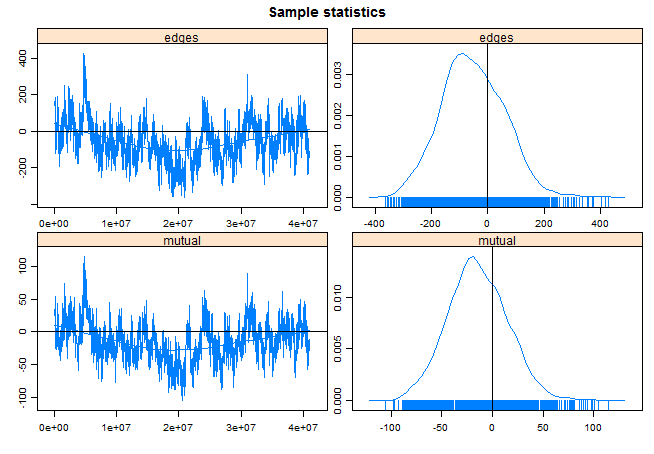
\includegraphics[width=0.8\textwidth]{Grafiken/mcmc_diag1.png}
	\caption{MCMC Diagnose von Modell 1 (1996) - edges und mutual}
	\end{figure}
	
	\begin{figure}[h]
	\centering
		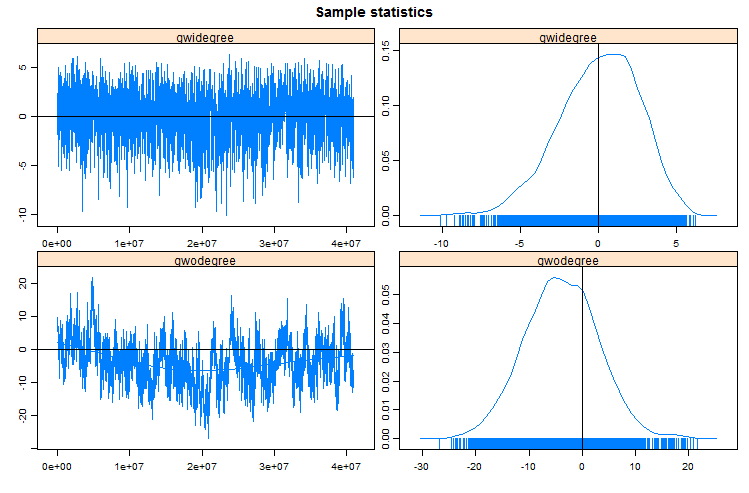
\includegraphics[width=0.8\textwidth]{Grafiken/mcmc_diag2.png}
	\caption{MCMC Diagnose von Modell 1 (1996) - gwidegree und gwodegree}
	\end{figure}
Beispielhaft aufgeführt sind hier die MCMC-Diagnosen der Statistiken \emph{edges, mutual, gwidegree} und \emph{gwodegree}. Bei allen vier Statistiken fällt die Diagnose zufriedenstellend aus. Es ist kein klarer Trend über die Ziehungen zu erkennen und die Werte der Statistiken schwanken nahezu symmetrisch um ihre Mittelwerte. Die MCMC-Diagnosen der restlichen im Modell 1 enthaltenen Statistiken ergeben ein ähnliches Ergebnis und sind hier deswegen nicht abgebildet.

\subsubsection{Goodness of Fit}
Nachdem die Funktion des Simulationsalgorithmus überprüft wurde, stellt sich nun die Frage ob das Modell auch die richtige Zielverteilung spezifiziert. Zu überprüfen gilt es also: Stimmen die gezogenen zufälligen Graphen aus der modellierten Verteilung mit dem beobachteten Graphen, der die Grundlage der Modellierung bildet, überein? Hierzu verwendet man sogenannte Goodness of Fit Plots. Den Statistiken aus zufällig gezogenen Graphen werden jene des beobachteten Graphen gegenübergestellt. Idealerweise sollten die Statistiken der gezogenen Graphen im Mittelwert mit den beobachteten Statistiken übereinstimmen oder diese zumindest überdecken. In Abbildung \ref{fig:gof.model1} sind die Goodness of Fit Plots für vier ausgewählte Statistiken abgebildet.

\begin{figure}[ht]
	\centering
		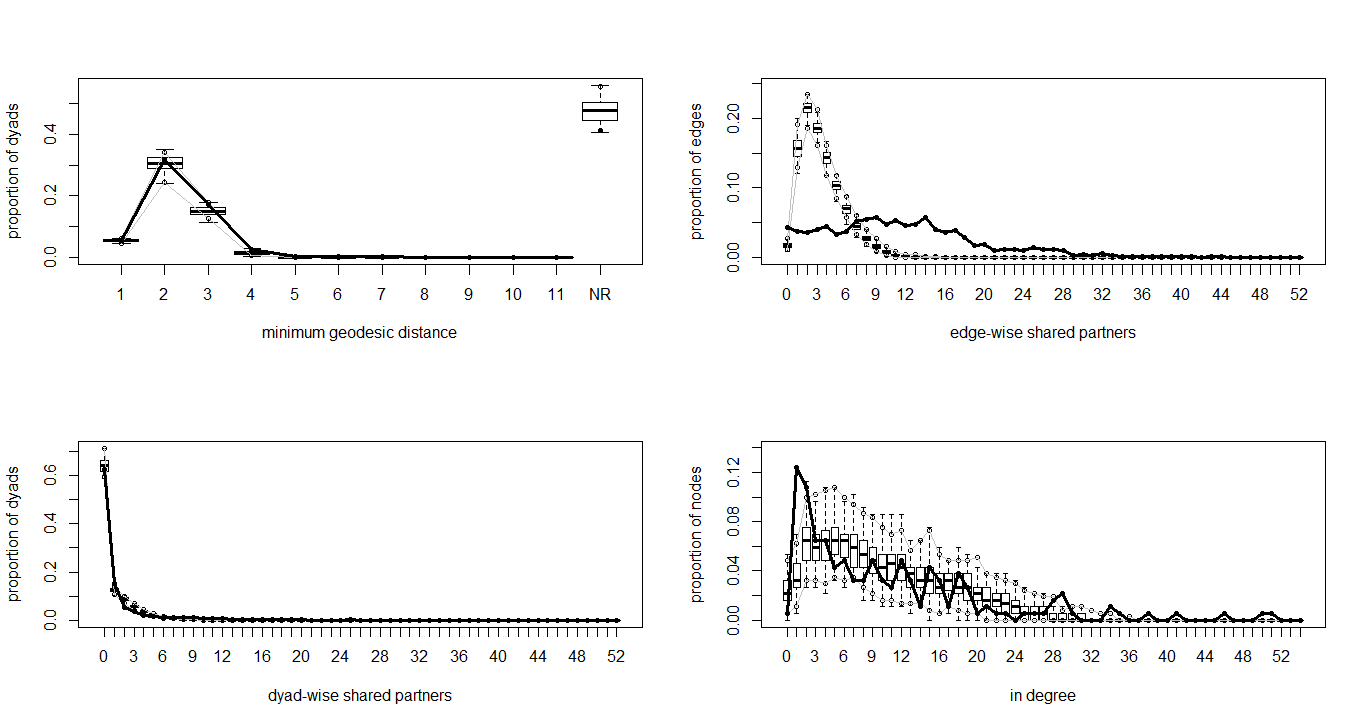
\includegraphics[width=0.9\textwidth]{Grafiken/GOF.png}
	\caption{Goodness of Fit von Modell 1 (1996)}
	\label{fig:gof.model1}
\end{figure}
Die \emph{Minimum Geodesic Distance} Statistik gibt den Anteil an Knotenpaaren an, deren Abstand einen bestimmten Wert annimmt. Aus der entsprechenden Grafik in Abbildung \ref{fig:gof.model1} geht zum Beispiel hervor, dass sowohl in dem beobachteten Graph als auch in den simulierten Graphen circa $30\%$ aller Knotenpaare einen Abstand von 2 besitzen und, dass fast die Hälfte aller Knotenpaare nicht miteinander verbunden ist.  Die schwarze Linie, die die Statistiken des beobachteten Graphen repräsentiert, liegt innerhalb der grauen Boxplots, die die Statistiken der simulierten Graphen darstellen. Das bedeutet also, dass unser Modell die Statistik \emph{Minimum Geodesic Distance} gut getroffen hat, obwohl sie nicht explizit in das Modell mit aufgenommen wurde.

Ebenfalls gut getroffen scheinen die Statistiken \emph{In Degree} und \emph{Dyad-wise shared Partners}. Erstaunlich schlecht getroffen ist die Statistik der \emph{Edge-wise shared Partners}. Obwohl diese über den Term \emph{gwesp} explizit in unser Modell mit aufgenommen wurde, liegen hier die Werte der beobachteten und simulierten Statistiken weit auseinander. Der Anteil an Kanten mit einer geringen Anzahl an gemeinsamen Partnern wird in unserem Modell weit überschätzt. Mögliche Gründe hierfür und weitere Probleme bei der Modellierung des Datensatzes werden im nächsten Abschnitt diskutiert.

\section{Probleme der Modellierung}
 Wie im letzten Abschnitt beschrieben, scheitert das Modell 1 bei der Modellierung der \emph{Edge-wise shared Partners} Statistik, obwohl diese in unser Modell mit aufgenommen wurde. Eine bessere, flachere Schätzung könnte eventuell durch einen kleineren Decay-Parameter erreicht werden. Hier stößt man allerdings auf ein entscheidendes Problem der Modellierung. Bereits kleine Variationen des Decay-Parameters führen zur Degeneration des Modells. Das gleiche Problem kann man bei der Variation des verwendeten Jahres und der verwendeten Statistiken beobachten. Das hier vorgestellte Modell 1 lässt sich nur in zwei der zwanzig im Datensatz enthaltenen Jahren anpassen, während es in allen anderen Jahren degeneriert. Eine Vielzahl von alternativen Variationen des Modells führen ebenfalls zur Degeneration oder zu wesentlich schlechteren Ergebnissen.

In Abschnitt \ref{sec:degeneration} wurde erklärt, dass die Degeneration eines Modells gleichbedeutend mit der schlechten Spezifikation eines Modells ist. Offensichtlich ist es also nicht gelungen, diejenige Kombination von endogenen und exogenen Statistiken zu finden, die den vorliegenden Datensatz adäquat beschreibt. Da diese aber nicht allein durch theoretische Überlegungen sondern vielmehr durch Ausprobieren verschiedenster Kombinationen zu ermitteln wäre, konnte dies im Rahmen dieser Arbeit schon aus rein zeitlichen Gründen nicht durchgeführt werden. Eine wünschenswertee freie Schätzung der Decay-Parameter und die Einbindung von zusätzlichen Knoten und Kantenattributen scheiterte zudem an den zum Teil sehr langen Rechenzeiten, die durch komplexere Modelle verursacht werden.

\section{Vergleich mit Modell des Großwaffenhandels}
Eine Vorgängerarbeit, die ebenfalls im Rahmen des Statistischen Consultings an der LMU angefertigt wurde, beschäftigte sich mit der Netzwerkanalyse des internationalen Großwaffenhandels \citep{js14}. Wunsch des Projektpartners ist es, die Ergebnisse der deskriptiven Analyse dieser Arbeit mit der Vorgängerarbeit zu vergleichen. Zudem soll die inzwischen weiterentwickelte Modellierung, die bei den Großwaffen hervorragende Ergebnisse erzielt, auf den Datensatz der Kleinwaffen übertragen werden, um eventuelle strukturelle Unterschiede zwischen den Handel mit Großwaffen und dem Handel mit kleinen und leichten Waffen  festzustellen. Die in der deskriptiven Analyse festgestellten Unterschiede sind in Tabelle \ref{tab:unterschiede} zusammengefasst.
\begin{table}[h]
		\centering
			\begin{tabular}{|l|c|c|}
				\hline
				Merkmal & Großwaffen & Kleinwaffen \\
				\hline
				\textbf{Zeitraum} & 1950 -2012 & 1992 -2011 \\
				\textbf{Anzahl Nationen} & 218 & 239 \\
				\textbf{Anzahl Transaktionen} &ca. 300-400 pro Jahr &ca. 4000-7000 pro Jahr\\
				\textbf{Dichte} & 0.025 - 0.035& 0.045 - 0.065\\
				\hline
			\end{tabular}
			\label{tab:unterschiede}
			\caption{Unterschiede der Datensätze zu Großwaffen und Kleinwaffen}
	\end{table}
Der Datensatz der Großwaffen stammt vom \emph{Stockholm International Peace Research Institute (SIPRI)} \footnote{\URL{http://www.sipri.org/}}. Er enthält den Zeitraum von 1950 bis 2012, während der Datensatz der Kleinwaffen lediglich den Zeitraum zwischen 1992 und 2011 abdeckt. Das Netzwerk des Großwaffenhandels enthält mit 218 beteiligten Nationen weniger als das Netzwerk des Kleinwaffenhandels mit 239 Nationen. Der größte Unterschied liegt jedoch in der Anzahl der Transaktionen. Während pro Jahr nur von etwa 300 bis 400 Transaktionen mit Großwaffen berichtet wird, enthält der Datensatz der Kleinwaffen pro Jahr zwischen 4000 und 7000 Transaktionen.

Beiden Datensätze ist gemein, dass die Degreeverteilung der Netzwerke auf einige zentrale Akteure schließen lässt, die in beiden Datensätzen größtenteils aus westlichen Industrienationen bestehen. Außerdem zeigt sich sowohl beim Handel mit Großwaffen als auch beim Handel mit Kleinwaffen im vergleichbaren Zeitraum ein ansteigender Trend bei der Anzahl der Transaktionen, der Anzahl der daran beteiligten Länder und des gehandelten monetären Volumens.

Die Modellierung des Datensatzes über den Großwaffenhandel wurde seit der Veröffentlichung von \citet{js14} weiterentwickelt und erzielt hervorragende Ergebnisse in Hinsicht auf den Goodness of Fit. Die Ergebnisse der Modellierung stehen kurz vor der Veröffentlichung. Im elektronischen Anhang befindet sich eine vorläufige Version des geplanten Artikels \citep{armstransfer}.

Beim Versuch, das Modell auf den Datensatz über kleine und leichte Waffen zu übertragen, stellt man jedoch fest, dass auch dieses Modell in allen 20 Jahren degeneriert. Daraus lässt sich dennoch schließen, dass es zwischen den Handel mit Großwaffen und dem mit Kleinwaffen strukturelle Unterschiede gibt, die die Modellierung mit identischen Statistiken verhindern.

\chapter{Diskussion}

Im Rahmen dieser Arbeit wurde mit Hilfe von Methoden der statistischen Netzwerkanalyse ein Datensatz des Peace Research Institute Oslo über den Handel mit kleinen und leichten Waffen in den Jahren 1992 bis 2011 untersucht.

Im Rahmen der deskriptiven Analyse wurde festgestellt, dass der Handel von einigen zentralen Akteuren dominiert wird. Hierbei handelt es sich vor allem um westliche Industrienationen. Das komplette Netzwerk lässt sich aufgrund seiner Größe schlecht übersichtlich visualisieren, weshalb die am Waffenhandel beteiligten Länder anhand der Kontinente in Gruppen aufgeteilt wurden. Aus der daraus resultierenden Darstellung geht Europa als derjenige Kontinent hervor, der am meisten Waffentransaktionen abwickelt. Die aus dem Handel resultierenden Geldströme variieren allerdings ohne erkennbares Muster zwischen den Kontinenten.

Die Modellierung des Netzwerkes mit Hilfe des Exponential Random Graph Modells erwies sich als schwierig. Ein geschätztes Modell für das Jahr 1996 erzielte zwar recht gute Ergebnisse, konnte aber nicht alle Aspekten das beobachtete Netzwerk korrekt abbilden. Die Instabilität des Modells bezüglich Variation des Decay-Parameters, des verwendeten Jahres und der verwendeten Statistiken lässt auf eine unzureichende Modellierung schließen. Eine weitere Optimierung des Modells scheitert an der zeitlichen Begrenzung dieses Projektes.

Ansätze zur weiteren Verbesserung sind allerdings durchaus vorhanden. Aus der Modellierung des Großwaffenhandels sind weitere Kovariablen verfügbar, die auch in der Modellierung der Kleinwaffenhandels Anwendung finden könnten. Dazu zählen insbesondere potenzielle Kantenattribute wie ein Datensatz über das internationale Bündnissystem oder auch die Mitgliedschaft in elitären wirtschaftlichen oder politischen Verbindungen wie dem G7-Bündnis.
Für eine korrekte Einbindung der exogenen Kovariablen wäre zudem eine deskriptive Betrachtung ihrer Eigenschaften nützlich.
Mit genügend Zeit und Geduld könnte man das Modell durch einfaches Ausprobieren von zahlreichen möglichen Kombinationen der endogenen Statistiken und des Decay-Parameters optimieren. Ein weiterer möglicher Ansatz zur Vermeidung langer Rechenzeiten wäre, mit der Modellierung von kleineren Teilnetzwerken zu beginnen, um von deren Eigenschaften eventuell Rückschlüsse auf das gesamte Netzwerk ziehen zu können.

Bisher keine Beachtung geschenkt wurde der zeitlichen Struktur der vorliegenden Netzwerkdaten. Dies könnte mit Hilfe einer alternativen Modellierung geschehen. Das \emph{Temporal Exponential Random Graph Modells} erlaubt die Einbindung von zeitlichen Effekten in die Modellierung und erzielt in \citet{armstransfer} vielversprechende Ergebnisse. 



\newpage







\bibliographystyle{dcu}
\bibliography{literatur}
\newpage
\listoffigures
\newpage
\listoftables




\chapter*{Kommentare zum elektronischen Anhang}
Die Inhalte des elektronischen Anhangs werden hier kurz erklärt: Er ist in folgende Ordner unterteilt:
\begin{itemize}
	\item \textbf{Arbeiten zum Großwaffendatensatz:} Dieser Ordner enthält den Bericht und den Vortrag der im Rahmen der Vorgängerarbeit erstellt wurde. Außerdem findet sich hier auch eine Vorabversion des Artikels, der die weiterentwickelte Modellierung des Großwaffendatensatzes beschreibt.
	\item \textbf{Bericht und Vortrag}: Dieser Ordner enthält den diesen Bericht und die dazugehörigen Vortragsfolien in elektronischer Form.
	\item \textbf{Importdaten}: Dieser Ordner enthält den verwendeten Datensatz des PRIO Institutes sowie die verwendeten Datensätze der exogenen Kovariablen.
	\item \textbf{R-Code}: Dieser Ordner enthält den lauffähigen und kommentierten R-Code mit dessen Hilfe die berichteten Analysen erstellt wurden. Zum Einlesen der Prio-Daten sollte die Datei \texttt{read-in.R} verwendet werden. Die Codes zum Einlesen der exogenen Kovariablen finden sich im Unterordner "`Kovariablen"'. Im Unterordner ERGM finden sich verschiedene ausprobierte Modelle, die durch die Datei \texttt{ergm-vorbereitung.R} lauffähig werden. Die anderen beiden Unterordner enthalten Code mit dessen Hilfe die im Bericht verwendeten Grafiken erstellt werden können und einige nützliche zusätzliche Funktionen die im Programmcode selbst ausreichend erklärt sind.
	\item \textbf{Sonstiges}: Dieser Ordner enthält eine Liste der aus dem Datensatz gelöschten Schleifen und der COW country codes.
\end{itemize} 


\chapter*{Eidesstattliche Erklärung}

Ich erkläre hiermit, dass ich diese Arbeit ohne fremde Hilfe angefertigt und nur die im Literaturverzeichnis aufgeführten Quellen und Hilfsmittel benutzt habe. Diese Arbeit wurde noch nicht zu anderen prüfungsrelevanten Zwecken vorgelegt.\\[1.5cm]

\noindent ..............................................
\qquad\qquad\qquad\qquad\qquad
....................................................\\[0.5mm]
\textit{Ort, Datum}
\qquad\qquad\qquad\qquad\qquad\qquad\qquad\qquad\qquad
\textit{Felix Loewe}














\end{document}


